\begin{enumerate}[label=\thesubsection.\arabic*.,ref=\thesubsection.\theenumi]
\item     Balance the following chemical equation.
    \begin{align}
        \label{eq:solutions/chem/6ato balance} HNO_{3}+ Ca(OH)_{2}\to Ca(NO_{3})_{2}+H_{2}O
    \end{align}
\solution
Let the balanced version of (\ref{eq:solutions/chem/6ato balance}) be
\begin{align}
    \label{eq:solutions/chem/6abalanced}x_{1}HNO_{3}+ x_{2}Ca(OH)_{2} \to x_{3}Ca(NO_{3})_{2}+ x_{4}H_{2}O
\end{align}
which results in the following equations:
\begin{align}
    (x_{1}+ 2x_{2}-2x_{4}) H= 0\\
    (x_{1}-2x_{3}) N= 0\\
    (3x_{1}+ 2x_{2}-6x_{3}- x_{4}) O=0\\
    (x_{2}-x_{3}) Ca= 0
\end{align}
which can be expressed as
\begin{align}
    x_{1}+ 2x_{2}+ 0 x_{3} -2x_{4} = 0\\
    x_{1}+ 0 x_{2} -2x_{3} +0.x_{4}= 0\\
    3x_{1}+ 2x_{2}-6x_{3}- x_{4} =0\\
    0 x_{1} +x_{2}-x_{3} +0.x_{4}= 0
\end{align}
resulting in the matrix equation
\begin{align}
    \label{eq:solutions/chem/6a matrix}
    \myvec{1 & 2 & 0 & -2\\
           1 & 0 & -2 & 0\\
           3 & 2 & -6 & -1\\
           0 & 1 & -1 & 0}\vec{x}
           =\vec{0}, \quad
   \vec{x}= \myvec{x_{1}\\x_{2}\\x_{3}\\x_{4}}
\end{align}
%
\eqref{eq:solutions/chem/6a matrix} can be reduced as follows
\begin{align}
    \myvec{1 & 2 & 0 & -2\\
           1 & 0 & -2 & 0\\
           3 & 2 & -6 & -1\\
           0 & 1 & -1 & 0}
    \xleftrightarrow[R_{3}\leftarrow \frac{R_3}{3}-R_{1}]{R_{2}\leftarrow R_2- R_1}
    \myvec{1 & 2 & 0 & -2\\
           0 & -2 & -2 & 2\\
           0 & -\frac{4}{3} & -2 & \frac{5}{3}\\
           0 & 1 & -1 & 0}\\
    \xleftrightarrow{R_2 \leftarrow -\frac{R_2}{2}}
    \myvec{1 & 2 & 0 & -2\\
          0 & 1 & 1 & -1\\
          0 & -\frac{4}{3} & -2 & \frac{5}{3}\\
          0 & 1 & -1 & 0}
    \xleftrightarrow[R_4 \leftarrow R_4- R_2]{R_3 \leftarrow R_3 + \frac{4}{3}R_2}
    \myvec{1 & 2 & 0 & -2\\
           0 & 1 & 1 & -1\\
           0 & 0 & -\frac{2}{3} & \frac{1}{3}\\
           0 & 0 & -2 & 1}\\
    \xleftrightarrow[R_3 \leftarrow -\frac{3}{2}R_3]{R_1 \leftarrow R_1- 2R_2}
    \myvec{1 & 0 & -2 & 0\\
           0 & 1 & 1 & -1\\
           0 & 0 & 1 & -\frac{1}{2}\\
           0 & 0 & -2 & 1}
    \xleftrightarrow{R_4\leftarrow R_4 + 2R_3}
    \myvec{1 & 0 & -2 & 0\\
           0 & 1 & 1 & -1\\
           0 & 0 & 1 & -\frac{1}{2}\\
           0 & 0 & 0 & 0}\\
    \xleftrightarrow[R_2\leftarrow R_2-R_3]{R_1\leftarrow R_1 + 2R_3}
    \myvec{1 & 0 & 0 & -1\\
           0 & 1 & 0 & -\frac{1}{2}\\
           0 & 0 & 1 & -\frac{1}{2}\\
           0 & 0 & 0 & 0}
\end{align}
Thus,
\begin{align}
    x_1=x_4, x_2= \frac{1}{2}x_4, x_3=\frac{1}{2}x_4\\
    \implies \quad\vec{x}= x_4\myvec{1\\[1ex] \frac{1}{2}\\[1ex] \frac{1}{2}\\[1ex]1} =\myvec{2\\1\\1\\2} 
\end{align} 
by substituting $x_4= 2$.
Hence, \eqref{eq:solutions/chem/6abalanced} finally becomes
\begin{align}
    2HNO_{3}+ Ca(OH)_{2}\to Ca(NO_{3})_{2}+ 2H_{2}O
\end{align}

%
\item    Balance the following chemical equation.
    \begin{align}
        \label{eq:solutions/chem/7b1} \text{Zinc + Silver nitrate} \to \text{Zinc nitrate + Silver}
    \end{align}
\solution
\eqref{eq:solutions/chem/7b1}  can be written as 
\begin{align}
\label{eq:solutions/chem/7b2} Zn+ AgNO_{3} \to Ag + Zn(NO_{3})_{2}
\end{align}
Suppose the balanced form of the equation is 
\begin{align}
    \label{eq:solutions/chem/7b3} x_{1}Zn+ x_{2}AgNO_{3} \to x_{3}Ag + x_{4} Zn(NO_{3})_{2},
\end{align}
which results in the following equations:
\begin{align}
    ( x_{1} - 2x_{4} ) Zn = 0\\
    ( x_{2} - x_{3} ) Ag = 0\\
    ( x_{3} - 2 x_{4} ) N =0\\
    ( 3x_{3} - 6x_{4} ) O = 0
\end{align}
which can be expressed as
\begin{align}
    x_{1} + 0 x_{2} + 0 x_{3} - x_{4} = 0\\
    0 x_{1} + x_{2} - x_{3} + 0 x_{4} = 0\\
    0 x_{1} + 0 x_{2} + x_{3} - 2 x_{4} =0\\
    0 x_{1} + 0 x_{2} + 3x_{3} - 6 x_{4}= 0
\end{align}
resulting in the matrix equation
\begin{align}
    \label{eq:solutions/chem/7b: matrix}
    \myvec{1 & 0 & 0 & -1\\
           0 & 1 & -1 & 0\\
           0 & 0 & 1 & -2\\
           0 & 0 & 3 & -6 }\vec{x}
           =\vec{0},\
   \vec{x}= \myvec{x_{1}\\x_{2}\\x_{3}\\x_{4}}
\end{align}
\eqref{eq:solutions/chem/7b: matrix} can be reduced as
\begin{align}
    \myvec{1 & 0 & 0 & -1\\
   	0 & 1 & -1 & 0\\
   	0 & 0 & 1 & -2\\
   	0 & 0 & 3 & -6 }
    \xleftrightarrow {R_{4}\leftarrow R_4 - 3R_3}
      \myvec{1 & 0 & 0 & -1\\
    	0 & 1 & -1 & 0\\
    	0 & 0 & 1 & -2\\
    	0 & 0 & 0 & 0 }
    \end{align}
Thus,
\begin{align}
    x_1 = x_4, x_ 2 = 2x_4, x_3 = 2x_4
    \implies \quad\vec{x } = \myvec{x_{4} \\ 2x_{4}\\ 2x_{4} \\ x_{4}}   =  x_4 \myvec{1\\ 2 \\ 2 \\1} =
 \myvec{1\\ 2 \\ 2 \\1},\
x_4= 1
    \end{align} 
Hence, \eqref{eq:solutions/chem/7b3} finally becomes
\begin{align}
Zn + 2AgNO_{3} \to 2Ag + Zn(NO_{3})_{2}
\end{align}

\item Write the balanced chemical equations for the following reaction. 
\begin{align}
 BaCl_2 + K_2SO_4 \rightarrow BaSO_4 + KCl \label{eq:solutions/chemistry/7d:1}   
\end{align}
%\solution
%\begin{enumerate}[label=\thesection.\arabic*,ref=\thesection.\theenumi]
\numberwithin{equation}{enumi}
\numberwithin{figure}{enumi}
\numberwithin{table}{enumi}
\item 
\label{chapters/9/9/3/1}
\iffalse
\documentclass[journal,12pt,twocolumn]{IEEEtran}

\usepackage[utf8]{inputenc}
\usepackage{kvmap}
\usepackage{graphics} 

\usepackage{setspace}
\usepackage{gensymb}

\singlespacing


\usepackage{amsthm}

\usepackage{mathrsfs}
\usepackage{txfonts}
\usepackage{stfloats}
\usepackage{bm}
\usepackage{cite}
\usepackage{cases}
\usepackage{subfig}

\usepackage{longtable}
\usepackage{multirow}

\usepackage{enumitem}
\usepackage{mathtools}
\usepackage{steinmetz}
\usepackage{tikz}
\usepackage{circuitikz}
\usepackage{verbatim}
\usepackage{tfrupee}
\usepackage[breaklinks=true]{hyperref}
\usepackage{graphicx}
\usepackage{tkz-euclide}
\usepackage{float}

\usetikzlibrary{calc,math}
\usepackage{listings}
    \usepackage{color}                                            %%
    \usepackage{array}                                            %%
    \usepackage{longtable}                                        %%
    \usepackage{calc}                                             %%
    \usepackage{multirow}                                         %%
    \usepackage{hhline}                                           %%
    \usepackage{ifthen}                                           %%
    \usepackage{lscape}     
\usepackage{multicol}
\usepackage{chngcntr}

\DeclareMathOperator*{\Res}{Res}

\renewcommand\thesection{\arabic{section}}
\renewcommand\thesubsection{\thesection.\arabic{subsection}}
\renewcommand\thesubsubsection{\thesubsection.\arabic{subsubsection}}

\renewcommand\thesectiondis{\arabic{section}}
\renewcommand\thesubsectiondis{\thesectiondis.\arabic{subsection}}
\renewcommand\thesubsubsectiondis{\thesubsectiondis.\arabic{subsubsection}}


\hyphenation{op-tical net-works semi-conduc-tor}
\def\inputGnumericTable{}                                 %%

\lstset{
%language=C,
frame=single, 
breaklines=true,
columns=fullflexible
}
\begin{document}


\newtheorem{theorem}{Theorem}[section]
\newtheorem{problem}{Problem}
\newtheorem{proposition}{Proposition}[section]
\newtheorem{lemma}{Lemma}[section]
\newtheorem{corollary}[theorem]{Corollary}
\newtheorem{example}{Example}[section]
\newtheorem{definition}[problem]{Definition}

\newcommand{\BEQA}{\begin{eqnarray}}
\newcommand{\EEQA}{\end{eqnarray}}
\newcommand{\define}{\stackrel{triangle}{=}}
\newcommand\hlight[1]{\tikz[overlay, remember picture,baseline=-\the\dimexpr\fontdimen22\textfont2\relax]\node[rectangle,fill=blue!50,rounded corners,fill opacity = 0.2,draw,thick,text opacity =1] {$#1$};}
\bibliographystyle{IEEEtran}
\providecommand{\mbf}{\mathbf}
\providecommand{\pr}[1]{\ensuremath{\Pr\left(#1\right)}}
\providecommand{\qfunc}[1]{\ensuremath{Q\left(#1\right)}}
\providecommand{\sbrak}[1]{\ensuremath{{}\left[#1\right]}}
\providecommand{\lsbrak}[1]{\ensuremath{{}\left[#1\right.}}
\providecommand{\rsbrak}[1]{\ensuremath{{}\left.#1\right]}}
\providecommand{\brak}[1]{\ensuremath{\left(#1\right)}}
\providecommand{\lbrak}[1]{\ensuremath{\left(#1\right.}}
\providecommand{\rbrak}[1]{\ensuremath{\left.#1\right)}}
\providecommand{\cbrak}[1]{\ensuremath{\left\{#1\right\}}}
\providecommand{\lcbrak}[1]{\ensuremath{\left\{#1\right.}}
\providecommand{\rcbrak}[1]{\ensuremath{\left.#1\right\}}}
\theoremstyle{remark}
\newtheorem{rem}{Remark}
\newcommand{\sgn}{\mathop{\mathrm{sgn}}}
\providecommand{\abs}[1]{\left\vert#1\right\vert}
\providecommand{\res}[1]{\Res\displaylimits_{#1}} 
\providecommand{\norm}[1]{$\left\lVert#1\right\rVert$}
%\providecommand{\norm}[1]{\lVert#1\rVert}
\providecommand{\mtx}[1]{\mathbf{#1}}
\providecommand{\mean}[1]{E\left[ #1 \right]}
\providecommand{\fourier}{\overset{\mathcal{F}}{ \rightleftharpoons}}
%\providecommand{\hilbert}{\overset{\mathcal{H}}{ \rightleftharpoons}}
\providecommand{\system}{\overset{\mathcal{H}}{ \longleftrightarrow}}
	%\newcommand{\solution}[2]{\textbf{Solution:}{#1}}
\newcommand{\solution}{\noindent \textbf{Solution: }}
\newcommand{\cosec}{\,\text{cosec}\,}
\providecommand{\dec}[2]{\ensuremath{\overset{#1}{\underset{#2}{\gtrless}}}}
\newcommand{\myvec}[1]{\ensuremath{\begin{pmatrix}#1\end{pmatrix}}}
\newcommand{\mydet}[1]{\ensuremath{\begin{vmatrix}#1\end{vmatrix}}}
\numberwithin{equation}{subsection}
\makeatletter
\@addtoreset{figure}{problem}
\makeatother
\let\StandardTheFigure\thefigure
\let\vec\mathbf
\renewcommand{\thefigure}{\theproblem}
\def\putbox#1#2#3{\makebox[0in][l]{\makebox[#1][l]{}\raisebox{\baselineskip}[0in][0in]{\raisebox{#2}[0in][0in]{#3}}}}
     \def\rightbox#1{\makebox[0in][r]{#1}}
     \def\centbox#1{\makebox[0in]{#1}}
     \def\topbox#1{\raisebox{-\baselineskip}[0in][0in]{#1}}
     \def\midbox#1{\raisebox{-0.5\baselineskip}[0in][0in]{#1}}
\vspace{3cm}
\title{\textbf{Matrix Assignment - Line} }
\author{Surabhi Seetha}
\maketitle
\newpage
\bigskip
\renewcommand{\thefigure}{\theenumi}
\renewcommand{\thetable}{\theenumi}
Get Python code for the figure from 
\begin{lstlisting}
https://github.com/SurabhiSeetha/Fwciith2022/tree/main/Assignment%201/codes/src
\end{lstlisting}
Get LaTex code from
\begin{lstlisting}
https://github.com/SurabhiSeetha/Fwciith2022/tree/main/avr%20gcc
\end{lstlisting}
%
\section{Question-Class 9, Exercise 9.3, Q(1)}
\fi
In the Figure 
		\ref{fig:9/9/3/1},
$\vec{E}$ is any point on median $AD$ of a $\triangle ABC$. Show that 
\begin{align}
ar(ABE) = ar(ACE). 
		\label{eq:9/9/3/1}
\end{align}

	\begin{figure}[!h]
		\centering
 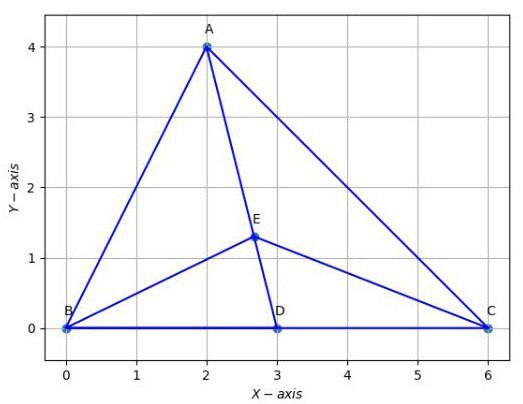
\includegraphics[width=\columnwidth]{chapters/9/9/3/1/figs/fig1.jpg}
		\caption{}
		\label{fig:9/9/3/1}
  	\end{figure}
	\begin{proof}
		From 
  \eqref{eq:area2d}
\begin{align}
	ar\brak{BDE}  
	& = 
 \frac{1}{2}\norm{\vec{B} \times \vec{D}+\vec{D} \times \vec{E}+\vec{E} \times \vec{B}}
 \\
	& = 
 \frac{1}{2}\norm{\vec{B} \times \brak{\frac{\vec{B}+\vec{C}}{2}}+\brak{\frac{\vec{B}+\vec{C}}{2}} \times \vec{E}+\vec{E} \times \vec{B}}
 \\
	& = 
 \frac{1}{4}\norm{\vec{B} \times \vec{C}+\vec{C} \times \vec{E}+\vec{E} \times \vec{B}}
  \end{align}
  after simplification.  Similarly, it can be shown that 
\begin{align}
	ar\brak{EDC} &= 
 \frac{1}{4}\norm{\vec{B} \times \vec{C}+\vec{C} \times \vec{E}+\vec{E} \times \vec{B}}
 \\
	&= ar\brak{BDE}
		\label{eq:9/9/3/1/1}
  \end{align}
The same approach can be used to show that
\begin{align}
	 ar\brak{ADB}
	= ar\brak{ADC}
		\label{eq:9/9/3/1/2}
  \end{align}
		Subtracting \eqref{eq:9/9/3/1/1}
from 
		\eqref{eq:9/9/3/1/2}
		yields
		\eqref{eq:9/9/3/1}

	\end{proof}
\iffalse

\centering
\includegraphics[width=0.45\textwidth]{Tri fig 1.jpg}
Figure 1 - Triangle ABC

\section{Construction}
\
\centering
\begin{tabular}{|c|c|c|}
\hline
\textbf{Symbol} & \textbf{Value} & \textbf{Description} \\
\hline
r & $\sqrt{20}$ & radius\\
\hline
$\theta$ & 63.45 & angle\\
\hline
B & $\begin{pmatrix} 0 \\ 0 \end{pmatrix}$ & Vertex B\\

\hline
C & $\begin{pmatrix}6 \\0 \end{pmatrix}$ & Vertex C\\
\hline

D & $\frac{B+C}{2}$ & Mid-point of BC\\
 
\hline

\end{tabular}

\centering
\begin{tabular}{|c|c|c|}

\hline

A & $\begin{pmatrix} rcos\theta \\ rsin\theta \end{pmatrix}$ & Vertex A\\

\hline

E & $\begin{pmatrix}Ex \\Ey \end{pmatrix}$ & point on AD\\

\hline

N & $\begin{pmatrix}Ax \\ 0 \end{pmatrix}$ & AN $\perp$ BC\\

\hline

M & $\begin{pmatrix}Ex \\ 0 \end{pmatrix}$ & EM $\perp$ BC\\

\hline

\end{tabular}

\section{Solution}
\raggedright{\subsection{Part-1:}}
We wish to show that
$Ar(\triangle ABE)=Ar(\triangle ACE)$\\
\vspace{0.25cm}
But to do so, firstly, we need to prove that $Ar(\triangle ABD)=Ar(\triangle ACD)$\\
\vspace{0.25cm}
Since the formula for area of a triangle is $\frac{1}{2}\times B \times H$, Let us draw an altitude $AN \perp BC$.\\
\
\begin{center}
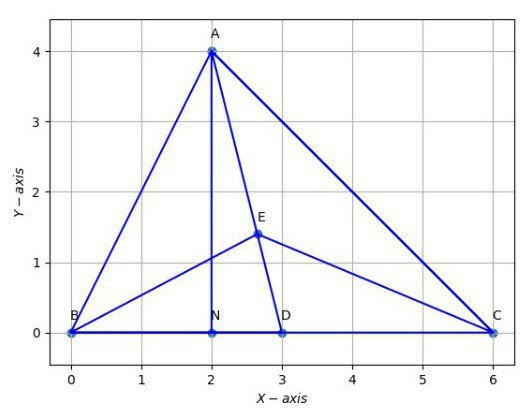
\includegraphics[width=0.4\textwidth]{Tri fig 2.jpg}\\
Figure 2 - $\triangle$ ABC with altitude ${AN} \perp {BC}$ \\
\end{center}

\hspace{0.1cm}Now, $Ar(\triangle ABD) = \frac{1}{2}$ $\times$ base $\times$ altitude of $\triangle ABD$\\
\centering
\vspace{0.25cm}
\hspace{1.6cm}$= \frac{1}{2}$ $\times$ $||{\vec{D-B}}||$ $\times$ $||{\vec{N-A}}||$\\
\vspace{0.25cm}
\
\hspace{2.9cm}\raggedright{$= \frac{1}{2}$ $\times$ $||{\vec{C-D}}||$ $\times$ $||{\vec{N-A}}||$} \vspace{0.25cm}\\
\hspace{3.5cm}{[$\because$ ${||\vec{D}-\vec{B}||}={||\vec{C}-\vec{D}||}$]}\\
\vspace{0.25cm}
\centering
\raggedright\hspace{3cm}$= \frac{1}{2}$ $\times$ base $\times$ altitude of $\triangle ACD$\\
\vspace{0.25cm}
\raggedright\hspace{2.95cm}{$=Ar(\triangle ACD)$}\\
\vspace{0.25cm}
\centering
\begin{align} 
\therefore Ar(\triangle ABD)=Ar(\triangle ACD) \hspace{0.25cm}
\label{eq:1}
\end{align}
\raggedright{\subsection{Part-2:}}

Next step is to show that $Ar(\triangle EDB)=Ar(\triangle EDC)$ by using the formula of area of a triangle.\\
\vspace{0.25cm}

To do so, now we need to draw another perpendicular from the point E onto the base $\overrightarrow{BC}$\\
\vspace{0.25cm}
\begin{center}
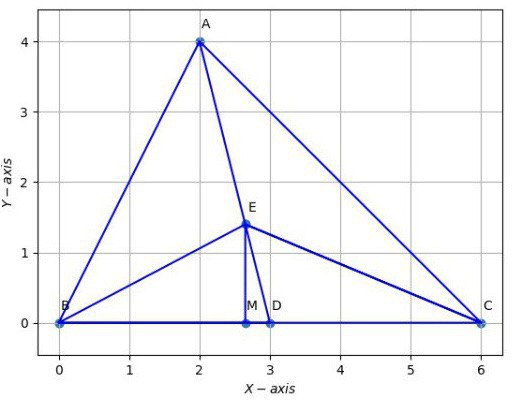
\includegraphics[width=0.4\textwidth]{Tri fig 3.jpg}\\
Figure 3 - $\triangle$ ABC with altitude ${EM} \perp {CB}$ \\
\end{center}

Now, $Ar(\triangle EDB) = \frac{1}{2}$ $\times$ base $\times$ altitude of $\triangle EDB$\\
\centering
\vspace{0.25cm}
\hspace{1.7cm}$= \frac{1}{2}$ $\times$ $||\vec{D-B}||$ $\times$ $||\vec{M-E}||$\\
\vspace{0.25cm}
\raggedright\hspace{3.0cm}{$= \frac{1}{2}$ $\times$ $||\vec{C-D}||$ $\times$ $||\vec{M-E}||$} \vspace{0.25cm}\\          
\hspace{3.5cm}{[$\because$ ${||\vec{D}-\vec{B}||}={||\vec{C}-\vec{D}||}$]}\\
\vspace{0.25cm}
\centering
\hspace{2.45cm}$= \frac{1}{2}$ $\times$ base $\times$ altitude of $\triangle EDC$\\
\vspace{0.25cm}
\raggedright\hspace{2.95cm}{$=Ar(\triangle ECD)$}\\

\centering
\begin{align}
\therefore Ar(\triangle EBD)=Ar(\triangle ECD) \hspace{0.25cm} 
\label{eqn:2}
\end{align}

\raggedright
From Fig.1, we can write that\\
\centering

\begin{align}
 Ar(\triangle ABD) = Ar(\triangle ABE) + Ar(\triangle EBD)\hspace{0.25cm} 
 \label{eqn:3}
\end{align}

\raggedright
And,
\begin{align}
Ar(\triangle ACD) = Ar(\triangle ACE) + Ar(\triangle ECD)\hspace{0.25cm} 
\label{eqn:4}
\end{align}
\raggedright
from the equation \ref{eq:1}, we can say that,
\centering
$$Ar(\triangle ABD)=Ar(\triangle ACD)$$.
\raggedright
Hence, from Eq.\ref{eqn:3} and eq.\ref{eqn:4} we get,\\
\vspace{0.25cm}
\raggedleft
\begin{align}
Ar(\triangle ABE) + Ar(\triangle EBD) =Ar(\triangle ACE) + Ar(\triangle ECD)
\end{align}
\vspace{0.25cm}
\raggedright
From eq. \ref{eqn:2}, we proved that\\
\centering
\vspace{0.25cm} 
$Ar(\triangle EBD)=Ar(\triangle ECD)$\\
\vspace{0.25cm}
\raggedright
Hence, from the above equations \ref{eqn:2} and \ref{eq:1} we can conclude that,\\
\vspace{0.25cm}
\centering
\begin{tabular}{|c|}
\hline
$\therefore$ Ar($\triangle$ ABE) = Ar($\triangle$ ACE)\\
\hline
\end{tabular}\\
\vspace{0.5cm}
Hence Proved

\end{document}
Footer
\fi


\item 
\label{chapters/9/9/3/2}
\iffalse
\documentclass[journal,10pt,twocolumn]{article}
\usepackage{graphicx}
\usepackage[margin=0.5in]{geometry}
\usepackage{amsmath}
\usepackage{array}
\usepackage{booktabs}
\usepackage{listings}
\providecommand{\norm}[1]{\left\lVert#1\right\rVert}
\providecommand{\abs}[1]{\left\vert#1\right\vert}
\usepackage{enumerate}
\let\vec\mathbf
\newcommand{\myvec}[1]{\ensuremath{\begin{pmatrix}#1\end{pmatrix}}}
\newcommand{\mydet}[1]{\ensuremath{\begin{vmatrix}#1\end{vmatrix}}}
\providecommand{\brak}[1]{\ensuremath{\left(#1\right)}}
\lstset{
frame=single,
breaklines=true,
columns=fullflexible
}
\title{\textbf{Matrix Assignment}}
\author{ALURU AJAY}
\date{September 2022}
\begin{document}
\maketitle

\section{Problem Statement}
\fi
In $\triangle ABC, \vec{E}$ is the mid-point of median $AD$.
Show that 
\begin{align}
ar(\triangle BED) = \frac{1}{4} ar(\triangle ABC)
		\label{eq:9/9/3/2}
\end{align}
	\begin{figure}[H]
		\centering
 \includegraphics[width=0.75\columnwidth]{chapters/9/9/3/2/figs/fig_Triangle.png}
		\caption{}
		\label{fig:9/9/3/2}
  	\end{figure}
\begin{proof}
	From Problem 
\ref{chapters/9/9/3/2},
  \begin{align}
ar(\triangle BED) =
 \frac{1}{4}\norm{\vec{B} \times \vec{C}+\vec{C} \times \vec{E}+\vec{E} \times \vec{B}}
		\label{eq:9/9/3/2/1}
  \end{align}
  Since 
  \begin{align}
	  \vec{E} &= \frac{ \vec{A}+\vec{D}}{2}
	  \\
	  &= \frac{ 2\vec{A}+\vec{B} + \vec{C}}{4},
  \end{align}
  substituting the above in 
		\eqref{eq:9/9/3/2/1}
		yields
  \begin{align}
	  ar(\triangle BED) &=
 \frac{1}{4}\norm{\vec{B} \times \vec{C}+\vec{C} \times \frac{ 2\vec{A}+\vec{B} + \vec{C}}{4}+\frac{ 2\vec{A}+\vec{B} + \vec{C}}{4} \times \vec{B}}
 \\
	  &=\frac{1}{8}\norm{\vec{A} \times \vec{B}+\vec{B} \times \vec{C}+\vec{C} \times \vec{A}}
  \end{align}
  resulting in
		\eqref{eq:9/9/3/2}.
\end{proof}
\iffalse

\section{Diagram}
Plot of Triangle is shown in figure 1, where point B is origin and points A, B, C and D are the vertices of Triangle.
\begin{figure}[H]
\includegraphics[width=0.75\columnwidth]{fig_Triangle.png}
\caption{Triangle}
\label{fig:Triangle}
\end{figure}
\section{PROOF}
In $\Delta ABC$,with AD as median
E is the mid-point of AD
\begin{center}
    $||{\vec{E-A}}||$ = $||{\vec{E-D}}||$
\end{center}
\begin{center}
\begin{equation}
    ||{\vec{D-B}}|| = \frac{1}{2} ||{\vec{C-B}}||
\end{equation}
\end{center}
\begin{flushleft}
From $\Delta ABC$
\end{flushleft}
\begin{equation}
    ar(\Delta ABC) = \frac{1}{2} \times ||{\vec{B-A}}|| \times ||{\vec{C-B}}||
\end{equation}
\begin{flushleft}
From $\Delta BED$
\vspace{0.3cm}\\
ar($\Delta BED$) = $\frac{1}{2}$ $\times$ $||{\vec{E-B}}||$ $\times$ $||{\vec{D-B}}||$
\vspace{0.3cm}\\
From Eq(1) we can write as
\begin{equation}
    ar(\Delta BED) = \frac{1}{2} \times ||{\vec{E-B}}|| \times\frac{1}{2} ||{\vec{C-B}}||
\end{equation}
We know that from Parallelogram law of Vector Addition
\begin{equation}
     \vec{E-B} = \frac{1}{2} ((\vec{B-A}) + \vec{C-B}))
\end{equation}
Substituting Eq(4) in Eq(3) $\And$ re-writing the Eq(3)\\
\vspace{0.3cm}
ar($\Delta BED$) = $\frac{1}{2}$ $\times$ (($\frac{1}{2}$$||{\vec{(B-A) + (C-B)}}||$) $\times$$\frac{1}{2}$ $||{\vec{C-B}}||$)
\vspace{0.5cm}\\
ar($\Delta BED$) = $\frac{1}{2}$ $\times$ $\frac{1}{4}$($||{\vec{B-A}}||$ $\times$ $||{\vec{C-B}}||$)
\vspace{0.5cm}\\
ar($\Delta BED$) =$\frac{1}{4}$ ($\frac{1}{2}$ $\times$ $||{\vec{B-A}}||$ $\times$ $||{\vec{C-B}}||$)
\vspace{0.5cm}\\
From Eq(2)
\vspace{0.3cm}\\
ar($\Delta BED$) =$\frac{1}{4}$(ar($\Delta ABC$)
\end{flushleft}
\vspace{0.5cm}
\centering
\begin{tabular}{|c|}
\hline
Ar($\Delta$ BED) = $\frac{1}{4}$ Ar($\Delta$ ABC)\\
\hline
\end{tabular}\\
\vspace{0.5cm}
Hence Proved

\begin{flushleft}
\section{Software}
\end{flushleft}
Download the codes given in the link below and execute them.\\
\begin{table}[H]
\centering
\begin{tabular}{|c|} \hline
\rule{0pt}{10pt} 
https://raw.githubusercontent.com/19PA1AO410/\\
FWC-Module-1/main/Matrix%20_Assignment/line_assignment/line.py
\\\hline
 \end{tabular}
\end{table}
\bibliographystyle{ieeetr}
\end{document}
\end{document}
\fi

\item 
\label{chapters/9/9/3/3}
\iffalse
\documentclass[journal,10pt,twocolumn]{article}
\usepackage{graphicx}
\usepackage[margin=0.5in]{geometry}
\usepackage{amsmath}
\usepackage{array}
\usepackage{booktabs}
\usepackage{listings}
\providecommand{\norm}[1]{\left\lVert#1\right\rVert}
\providecommand{\abs}[1]{\left\vert#1\right\vert}
\usepackage{enumerate}
\let\vec\mathbf
\newcommand{\myvec}[1]{\ensuremath{\begin{pmatrix}#1\end{pmatrix}}}
\newcommand{\mydet}[1]{\ensuremath{\begin{vmatrix}#1\end{vmatrix}}}
\providecommand{\brak}[1]{\ensuremath{\left(#1\right)}}
\lstset{
frame=single,
breaklines=true,
columns=fullflexible
}
\title{\textbf{Matrix Assignment}}
\author{Mannava Venkatasai}
\date{September 2022}
\begin{document}
\maketitle
\fi
 Show that the diagonals of a parallelogram divide
it into four triangles of equal area.
	\begin{figure}[!h]
		\centering
 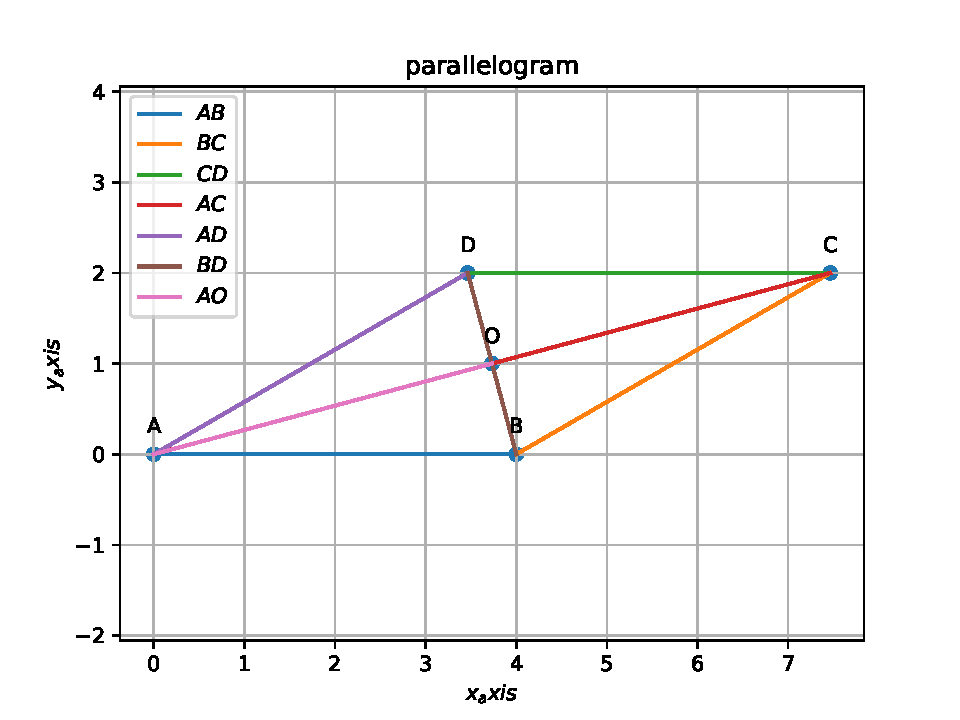
\includegraphics[width=\columnwidth]{chapters/9/9/3/3/figs/par.pdf}
		\caption{}
		\label{fig:9/9/3/3}
  	\end{figure}
\begin{proof}
	See Fig. 
		\ref{fig:9/9/3/3}.
	From Appendix
	  \ref{prop:two-pgm-diag-bisect} and 
  \ref{prop:area2d}
\begin{align}
	ar\brak{AOB} &= 
	\frac{1}{2} \norm{\vec{A} \times \vec{O}+\vec{O} \times \vec{B}+\vec{B} \times \vec{A}}
	\\
	&=	\frac{1}{2} \norm{\vec{A} \times \brak{\frac{\vec{A}+\vec{C}}{2}}+\brak{\frac{\vec{A}+\vec{C}}{2}} \times \vec{B}+\vec{B} \times \vec{A}}
	\\
	&=\frac{1}{4} \norm{\vec{A} \times \vec{C}+\vec{C} \times \vec{B}+\vec{B} \times \vec{A}}
  \end{align}
  yielding the desired result from Appendix
  \ref{prop:pgm2d}
\end{proof}
\iffalse
\begin{enumerate}
	\item AB=DC and AD=BC
	\item O is the midpoint of AC and BD
\end{enumerate}
\begin{figure}[h]
\centering
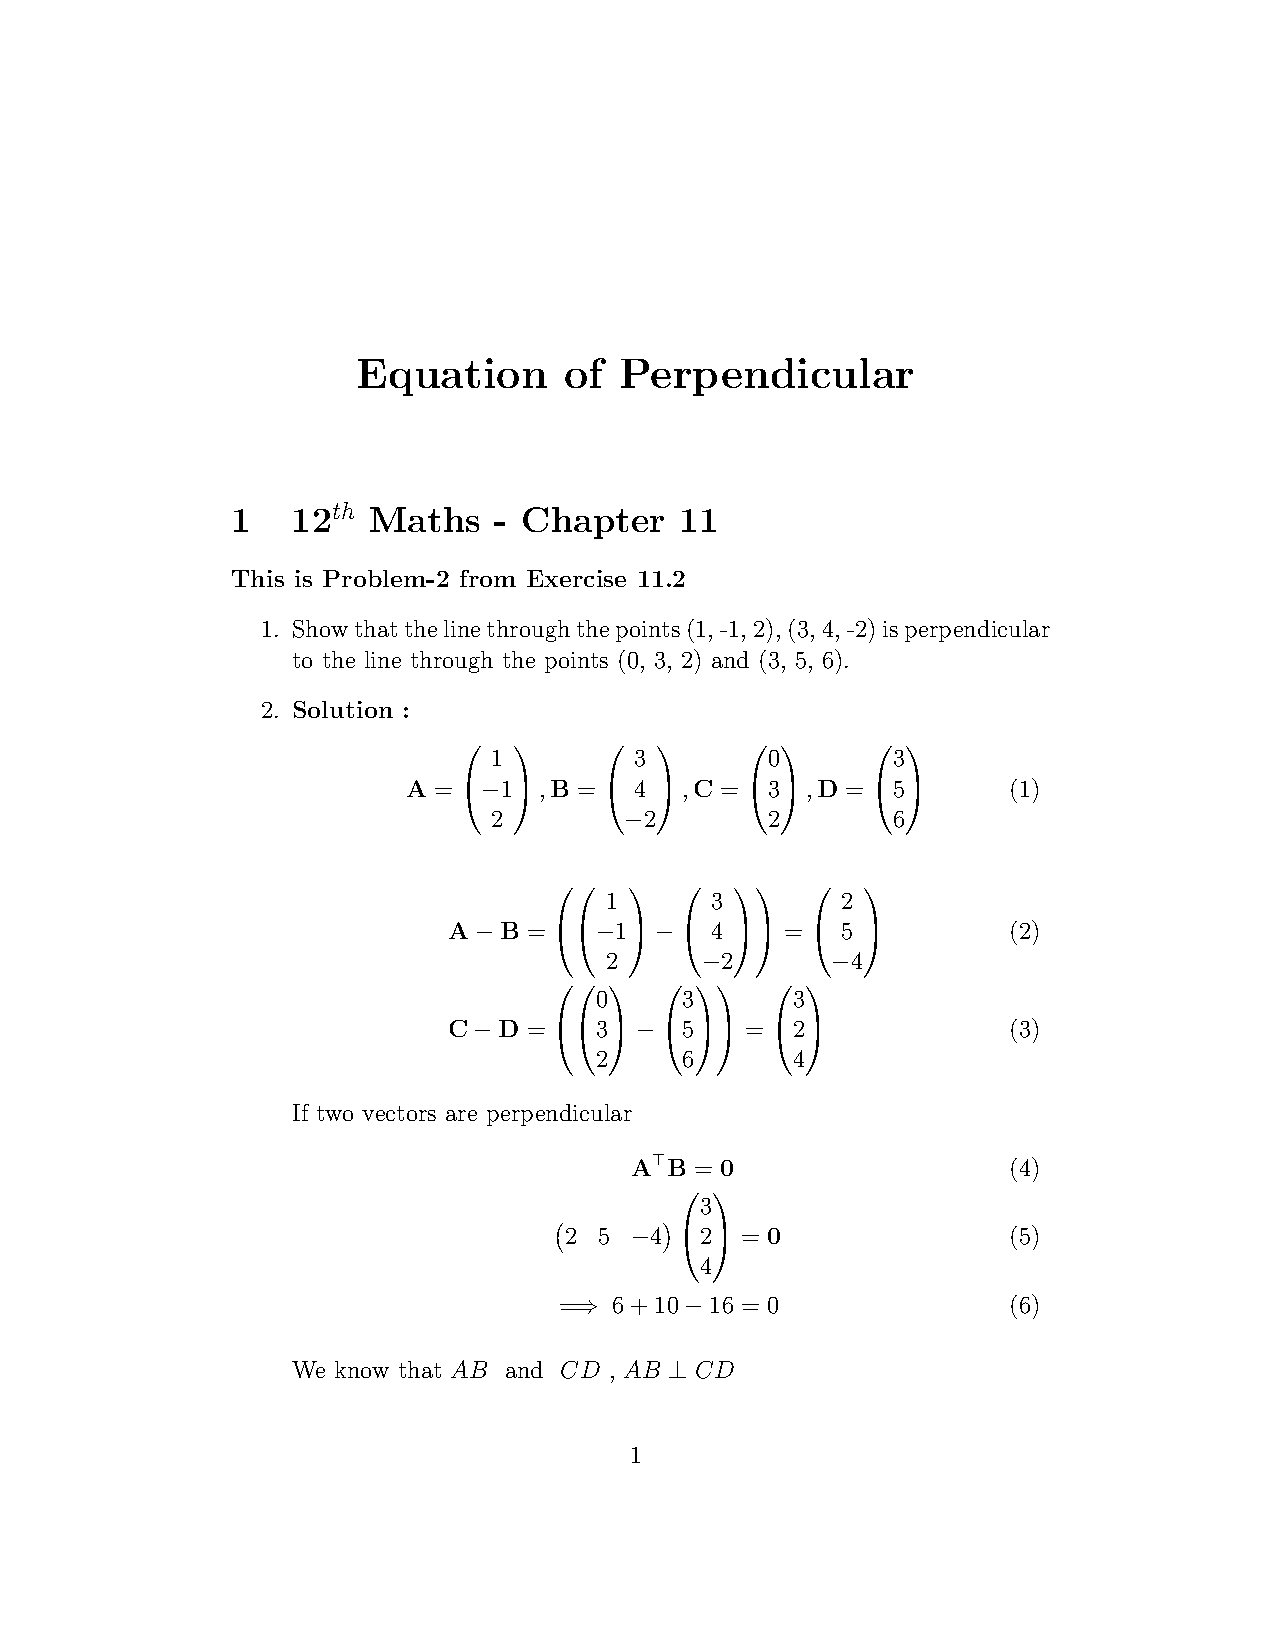
\includegraphics[width=1\columnwidth]{par.pdf}
\caption{Parallelogram ABCD With centre O}
\label{fig:Parallelogram}
\end{figure}

\section*{Solution}
\subsection*{Part 1}
\section*{Construction}
The input parameters are the lengths of AB and AD and angle between AB and ADs \vspace{2mm}\\
{
\setlength\extrarowheight{2pt}
\begin{tabular}{|c|c|c|}
	\hline
	\textbf{Symbol}&\textbf{Value}&\textbf{Description}\\
	\hline
	d&4&AB\\
	\hline
	r&3&AD\\
	\hline
	$\theta$&$\pi/6$&$\angle$A\\
	\hline
	\textbf{D}&$r%
	\begin{pmatrix}
		cos\theta\\
		sin\theta\\
	\end{pmatrix}$%
	&Point \textbf{D}\\
	\hline
	\textbf{C}&\textbf{B}+\textbf{D}
	&Point \textbf{C}\\
	\hline
\end{tabular}
}
\subsection*{Part 2}
The diagnols of a parallelogram bisect each other. 
\begin{align}
\vec{O-A} =\vec{C-O} 
\end{align}
\begin{align}
			\vec{O-D} =\vec{B-O} 
\end{align}
\begin{align}
	(\vec{C-A}) =(\vec{B-A}) + (\vec{C-B})
\end{align}
\begin{align}
	(\vec{B-D}) =(\vec{B-A}) - (\vec{C-B})
\end{align}
\begin{align}
	(\vec{O-A}) =(\vec{C-A})/2
\end{align}
\begin{align}
	(\vec{O-D}) =(\vec{B-D})/2
\end{align}
\textbf{In parallelogram ABCD} \vspace{2mm} \\
\begin{enumerate}[1.]
\item \textbf{consider $\triangle$ AOB}
\end{enumerate}
Area of triangle is given as 
\begin{align}
	\frac{1}{2}{\left | (\vec{O-A}\times\vec{B-O})\right |}
\end{align}
\begin{align}
	\frac{1}{2}{\left | (\vec{B-A})+(\vec{C-B})/2\times(\vec{B-A})-(\vec{C-B})/2\right |}
\end{align}
\begin{align}
	 \textbf{Area of $\triangle$AOB} = \frac{1}{4}{\left | (\vec{B-A})\times(\vec{C-B})\right |}
\end{align}
\vspace{5mm}
\begin{enumerate}[2.]
\item  \textbf{consider $\triangle$ BOC}
\end{enumerate}
Area of triangle is given as 
\begin{align}
	\frac{1}{2}{\left | (\vec{B-O})\times(\vec{C-O})\right |}
\end{align}
\begin{align}
	\frac{1}{2}{\left | ((\vec{B-A})-(\vec{C-B}))/2\times((\vec{B-A})+(\vec{C-B}))/2\right |}
\end{align}
\begin{align}
	\frac{1}{4}{\left | (\vec{B-A})\times(\vec{C-B})\right |}
\end{align}
\begin{align}
 \textbf{Area of $\triangle$BOC} = \frac{1}{4}{\left | (\vec{B-A})\times(\vec{C-B})\right |}
\end{align}
\vspace{5mm}
\begin{enumerate}[3.]
 \item \textbf{consider $\triangle$ COD}
\end{enumerate}
Area of triangle is given as \\
\begin{align}
	\frac{1}{2}{\left |(\vec{C-O})\times(\vec{D-O})\right |}
\end{align}
\begin{align}
	\frac{1}{4}{\left | (\vec{B-A})\times(\vec{C-B})\right |}
\end{align}
\begin{align}
\textbf{Area of $\triangle$COD} = \frac{1}{4}{\left | (\vec{B-A})\times(\vec{C-B})\right |}
\end{align}
\vspace{5mm}
\begin{enumerate}[4.]
\item \textbf{consider $\triangle$ DOA}
\end{enumerate}
Area of triangle is given as \\
\begin{align}
	\frac{1}{2}{\left |( \vec{A-O})\times(\vec{D-O})\right |}
\end{align}
\begin{align}
	\frac{1}{2}{\left | (-(\vec{B-A})-(\vec{C-B}))/2\times(-(\vec{B-A})+(\vec{C-B}))/2\right |}
\end{align}
\begin{align}
	\frac{1}{4}{\left | (\vec{B-A})\times(\vec{C-B})\right |}
\end{align}
\begin{align}
\textbf{Area of $\triangle$AOD} = \frac{1}{4}{\left | (\vec{B-A})\times(\vec{C-B})\right |}
\end{align}
Hence from the above results we can conclude that \vspace{3mm} \\
\textbf{ar($\triangle${AOB})=ar($\triangle${BOC})=ar($\triangle${COD})=ar($\triangle${DOA})\\= 1/4*${\left | \textbf{B-A}\times\textbf{C-B}\right |}$}  \vspace{4mm} \\
\textbf{Hence We prooved that the diagonals of a parallelogram divide it into 
four triangles of equal area.} \vspace{4mm} \\
\end{document}
\fi

\item 
\label{chapters/9/9/3/4}
\iffalse
\def\mytitle{MATRICES USING PYTHON}
\def\myauthor{P.kalyan}
\def\contact{kalyanpadyalaanirudh@gmail.com}
\def\mymodule{Future Wireless Communication (FWC)}
\documentclass[10pt, a4paper]{article}
\usepackage[a4paper,outer=1.5cm,inner=1.5cm,top=1.75cm,bottom=1.5cm]{geometry}
\twocolumn
\usepackage{graphicx}
\graphicspath{{./images/}}
\usepackage[colorlinks,linkcolor={black},citecolor={blue!80!black},urlcolor={blue!80!black}]{hyperref}
\usepackage[parfill]{parskip}
\usepackage{lmodern}
\usepackage{tikz}
	\usepackage{physics}
%\documentclass[tikz, border=2mm]{standalone}
\usepackage{karnaugh-map}
%\documentclass{article}
\usepackage{tabularx}
\usepackage{circuitikz}
\usetikzlibrary{calc}
\usepackage{amsmath}
\usepackage{amssymb}
\renewcommand*\familydefault{\sfdefault}
\usepackage{watermark}
\usepackage{lipsum}
\usepackage{xcolor}
\usepackage{listings}
\usepackage{float}
\usepackage{titlesec}
\providecommand{\mtx}[1]{\mathbf{#1}}
\titlespacing{\subsection}{1pt}{\parskip}{3pt}
\titlespacing{\subsubsection}{0pt}{\parskip}{-\parskip}
\titlespacing{\paragraph}{0pt}{\parskip}{\parskip}
\newcommand{\figuremacro}[5]{
    \begin{figure}[H]
        \centering
        \includegraphics[width=0.75\columnwidth]{#2}
        \caption[#3]{\textbf{#3}#4}
        \label{fig:#2}
    \end{figure}
}
\newcommand{\myvec}[1]{\ensuremath{\begin{pmatrix}#1\end{pmatrix}}}
\let\vec\mathbf
\lstset{
frame=single, 
breaklines=true,
columns=fullflexible
}

\thiswatermark{\centering \put(0,-90){
\includegraphics[width=0.75\columnwidth]{iith}} }
\title{\mytitle}
\author{\myauthor\hspace{1em}\\\contact\\FWC22031\hspace{6.5em}IITH\hspace{0.5em}\mymodule\hspace{6em}ASSIGN-5}
\date{}
\begin{document}
	\maketitle
	\tableofcontents
   \section{Problem}
   \fi
   $ABC, ABD$ are 2 triangles on same base $AB$, if line segment $CD$ is bisected by $AB$ at $\vec{O}$, show that 
   \begin{align}
		\label{eq:9/9/3/4}
 ar (ABC) = ar (ABD)  
   \end{align}
	\begin{figure}[H]
		\centering
 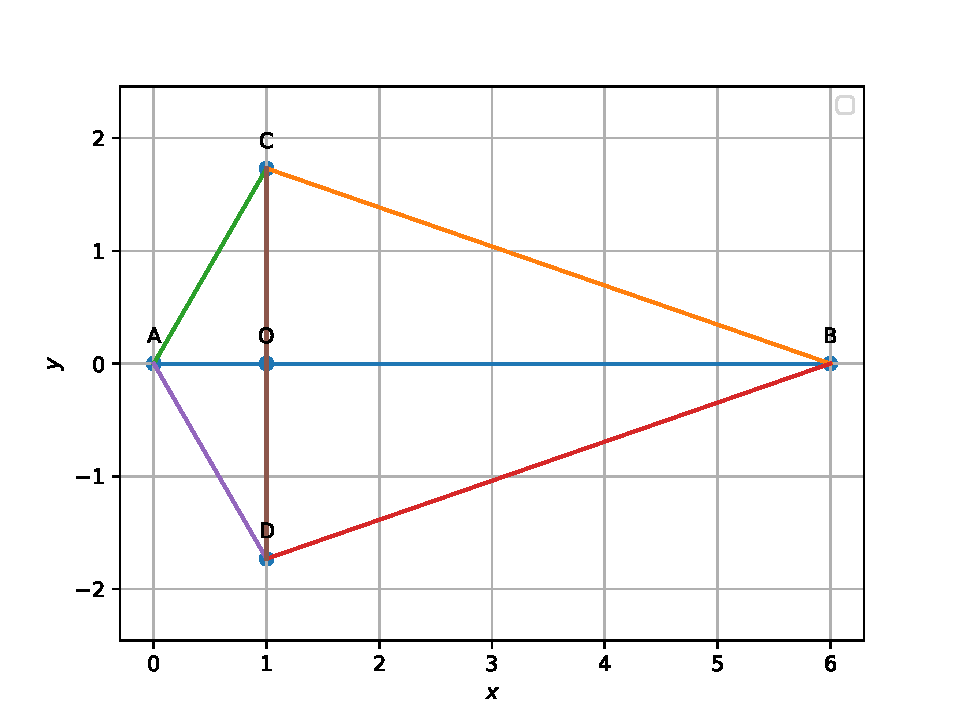
\includegraphics[width=0.75\columnwidth]{chapters/9/9/3/4/figs/figa6.pdf}
		\caption{}
		\label{fig:9/9/3/4}
  	\end{figure}
	\begin{proof}
		See Fig. 
		\ref{fig:9/9/3/4}. $AO$ and $OB$ are medians of triangles $ADC$ and $BDC$. From 
Appendix	  \ref{prop:two-median-area}, 
		\eqref{eq:9/9/3/4} is trivial.
	\end{proof}


\iffalse

	    \includegraphics[width=0.75\columnwidth]{}
   \section{Solution}
   \textbf{Theory:}\\
In 2 triangles with same base and linesegment cd is bisected at o  
\textbf{To Prove:} Ar(ABC)=Ar(ABD) \\
\textbf{Theorem} : Two triangles on the same base (or equal bases) and having the equal heights are equal in area.
\begin{center}
$\therefore$ Ar($\Delta$ ABC)=Ar($\Delta$ ABD)......(1)\\
Hence, Proved    
\end{center}


\
\textbf{termux commands :}
\begin{lstlisting}
python3 matrix.py
\end{lstlisting}


The input parameters for this construction are 
\begin{center}
\begin{tabular}{|c|c|c|}
	\hline
	\textbf{Symbol}&\textbf{Value}&\textbf{Description}\\
	\hline
	k1&4&length of CD\\
	\hline
	k2&6&length of AB\\
	\hline
 
	\hline
	O&$\
	\begin{pmatrix}
		0 \\
		0 \\
	\end{pmatrix}$%
	&Point O\\
	
	\hline
\end{tabular}
\end{center}
\textbf{To Prove:} Ar(ABC)=Ar(ABD)
  %	\begin{align}
	%		\vec{C} &= \myvec{0 \\ 0}, \vec{E}=\myvec{-5 \\ 3}\\
	%			\vec{F} &= \myvec{3 \\ 0}, \vec{D}=\myvec{-3 \\ 0}
	%	\end{align}
		\begin{center}
	a=A-B\\
	b=C-B\\
	c=B-D\\
	Area of the $\Delta$ABC is given by \\
Ar($\Delta$ABC) =$\frac{1}{2}$$\norm{\vec{a}\times\vec{b}}$............(2)\\
    b=C-B\\
	c=B-D\\
		Area of the $\Delta$ABD is given by \\
 Ar($\Delta$ABD) =$\frac{1}{2}$$\norm{\vec{c}\times\vec{d}}$...............(3)
	\end{center}
	
	\begin{center}
$\therefore$ Ar(ABC)=Ar(ABD)........(4)\\
	\end{center}
The below python code realizes the above construction:	
\begin{lstlisting}
https://github.com/anirudhkalyan/fwc
\end{lstlisting}
 \section{Construction}
 	\begin{center}
  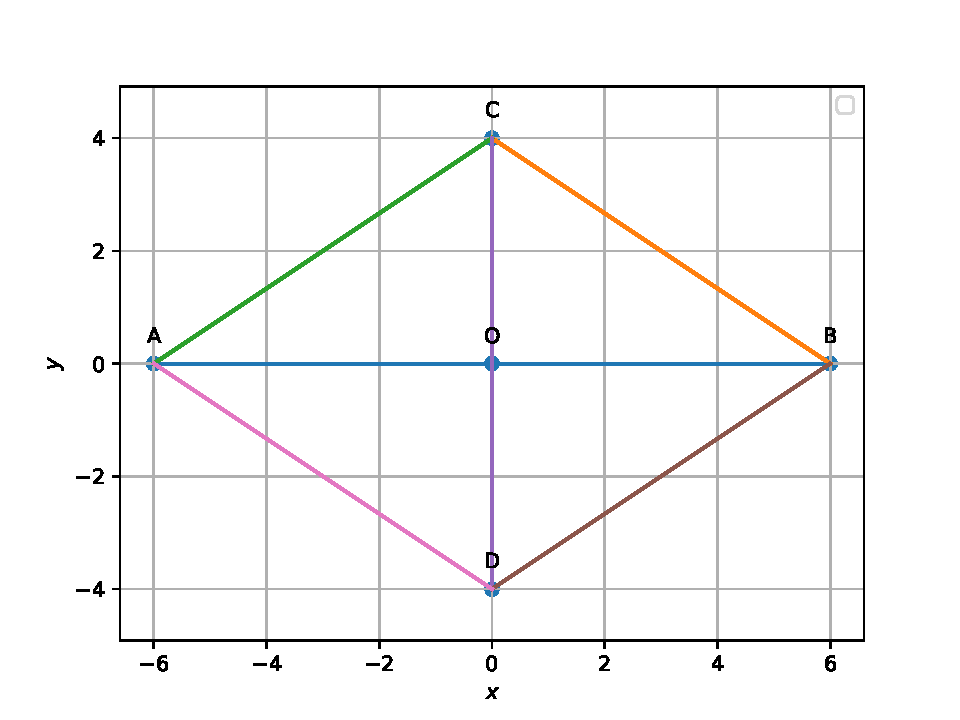
\includegraphics[width=0.75\columnwidth]{figsa1.pdf}
  
  Figure of construction
  	\end{center}
  	  
\bibliographystyle{ieeetr}
\end{document}
\fi

\item 
\item 
\item 
\item 

\item 
\label{chapters/9/9/3/9}
\iffalse
\documentclass[journal,10pt,twocolumn]{article}
\usepackage{graphicx}
\usepackage[margin=0.5in]{geometry}
\usepackage{array}
\usepackage{amsmath}
\usepackage{booktabs}
\title{\textbf{Line Assignment}}
\author{Alavala Chinnapa Reddy}
\date{September 2022}

\begin{document}

\maketitle
\fi
 The side $AB$ of a parallelogram $ABCD$ is produced to any point $\vec{P}$. A line through $\vec{A}$ and parallel to $CP$ meets $CB$ produced at $\vec{Q}$ and then parallelogram $PBQR$ is completed. Show that
 \begin{align}
	 ar(ABCD) = ar(PBQR)
		\label{eq:9/9/3/9}
 \end{align}
	\begin{figure}[!h]
		\centering
 \includegraphics[width=\columnwidth]{chapters/9/9/3/9/figs/l1.pdf}
		\caption{}
		\label{fig:9/9/3/9}
  	\end{figure}
	\begin{proof}
		From the given information, using section formula, 
  \begin{align}
		\label{eq:9/9/3/9/p}
	  \vec{Q}&= \frac{k_1\vec{C}+ \vec{B}}{k_1+1}
	  \\
	  \vec{P}&= \frac{k_2\vec{A}+ \vec{B}}{k_2+1}
		\label{eq:9/9/3/9/q}
  \end{align}
  Also, since $AQ \parallel CP$,
  \begin{align}
	  \vec{A}-\vec{Q}=k\brak{\vec{C}-\vec{P}}
  \end{align}
  Substituting from 
		\eqref{eq:9/9/3/9/p}
		and
		\eqref{eq:9/9/3/9/q}
		in the above, 
  \begin{align}
	  \vec{A}-\frac{k_1\vec{C}+ \vec{B}}{k_1+1}=k\brak{\vec{C}-\frac{k_2\vec{A}+ \vec{B}}{k_2+1}}
  \end{align}
  which, after some algebra, yields
  \begin{align}
		\label{eq:9/9/3/9/tri}
	  \brak{1 + \frac{kk_2}{k_2+1}}  \vec{A}+\brak{\frac{k}{k_2+1}-\frac{1}{k_1+1}}\vec{B}- \brak{\frac{k_1}{k_1+1}+k}\vec{C}=\vec{0}
  \end{align}
  From Appendix
	  \ref{prop:two-tri-indep},
		\eqref{eq:9/9/3/9/tri}
		results in
  \begin{align}
	  \brak{\frac{k}{k_2+1}-\frac{1}{k_1+1}} &=
	  \brak{\frac{k_1}{k_1+1}+k}= 0
	  \\
	  \text{or, } k_1 +k_2 = -1
		\label{eq:9/9/3/9/k1k2}
  \end{align}

From Appendix
  \ref{prop:pgm2d}
\begin{align}
	ar\brak{PBQR} &= \norm{\vec{P} \times \vec{B}+\vec{B} \times \vec{Q}+\vec{Q} \times \vec{P}}
		\label{eq:9/9/3/9/arpbqr}
  \end{align}
  The R.H.S. in the above can be expressed as
\begin{align}
\frac{k_2\vec{A}+ \vec{B}}{k_2+1} \times \vec{B}+\vec{B} \times \frac{k_1\vec{C}+ \vec{B}}{k_1+1}+\frac{k_1\vec{C}+ \vec{B}}{k_1+1} \times \frac{k_2\vec{A}+ \vec{B}}{k_2+1}
  \end{align}
  leading to 
  \begin{multline}
	  \brak{\frac{k_2}{k_2+1}-\frac{k_2}{\brak{k_1+1}\brak{k_2+1}}} \vec{A}\times \vec{B}
	  \\
	  +\vec{B} \times\vec{C}\brak{ \frac{k_1}{k_1+1}-\frac{k_1}{\brak{k_1+1}\brak{k_2+1}}}
	  \\
	  +\frac{k_1k_2}{\brak{k_1+1}\brak{k_2+1}}\vec{C} \times \vec{A}
  \end{multline}
  that can be simplified to obtain
\begin{align}
	ar\brak{PBQR} 
	  &=
	  \frac{k_1k_2}{\brak{k_1+1}\brak{k_2+1}}\norm{\brak{\vec{A} \times \vec{B}+\vec{B} \times \vec{C}+\vec{C} \times \vec{A}}}
	  \\
	  &=\norm{\brak{\vec{A} \times \vec{B}+\vec{B} \times \vec{C}+\vec{C} \times \vec{A}}}
		\label{eq:9/9/3/9/pbqr}
\end{align}
  using the fact that 
  \begin{align}
\frac{k_1k_2}{\brak{k_1+1}\brak{k_2+1}} = 1
  \end{align}
  from 
		\eqref{eq:9/9/3/9/k1k2}.  Also, from 
Appendix
  \ref{prop:pgm2d},
  \begin{align}
ar\brak{ABCD} = \norm{\brak{\vec{A} \times \vec{B}+\vec{B} \times \vec{C}+\vec{C} \times \vec{A}}}
		\label{eq:9/9/3/9/abcd}
  \end{align}
  yielding
		\eqref{eq:9/9/3/9} from 
		\eqref{eq:9/9/3/9/pbqr}.
	\end{proof}
\iffalse

\begin{figure}[h]
\centering
\includegraphics[width=1\columnwidth]{figs/l1.pdf}
\caption{parallelogram PBQR is produced using parallelogram ABCD}
\end{figure}

\section*{Solution}
\subsection*{METHOD 1}

Let 
\begin{equation}
\boldsymbol{B-A} = \boldsymbol{m}
\end{equation}
\begin{equation}
\boldsymbol{D-A} = \boldsymbol{n} 
\end{equation}
n written as two perpendicular components one along $\boldsymbol{m}$ and one perpendicular to $\boldsymbol{m}$
\begin{equation}
   \boldsymbol{n}=\boldsymbol{m} \parallel_A +\boldsymbol{m} \perp_A
\end{equation}
\begin{equation}
\boldsymbol{m} \parallel_A ={\frac{\boldsymbol{n}^T\boldsymbol{m}}{||\boldsymbol{m}||^2}}\boldsymbol{m}
\end{equation}
\begin{equation}
\boldsymbol{m} \perp_A =\boldsymbol{n} - \boldsymbol{m} \parallel_A
\end{equation}
\begin{equation}
\boldsymbol{m} \perp_A=\boldsymbol{n}-{\frac{\boldsymbol{n}^T\boldsymbol{m}}{||\boldsymbol{m}||^2}}\boldsymbol{m}
\end{equation}
\begin{equation}
||\boldsymbol{m} \perp_A||^2=||\boldsymbol{n}||^2-{\frac{{\boldsymbol{n}^2T\boldsymbol{m}}^2}{||\boldsymbol{m}||^2}}
\end{equation}
\begin{eqnarray}
    Area of parallelogram ABCD =\sqrt{{base}^2{height}^2}\\
    Area of parallelogram ABCD =\sqrt{{||\boldsymbol{m} \perp_A}||^2{||\boldsymbol{m}||^2}}\\
    Area of parallelogram ABCD =\sqrt{(||\boldsymbol{n}||^2-{\frac{{\boldsymbol{n}^2T\boldsymbol{m}}^2}{||\boldsymbol{m}||^2}})||\boldsymbol{m}||^2}
\end{eqnarray}
Let\\
Q lies on BC extended
\begin{eqnarray}
    \boldsymbol{P}=\boldsymbol{B}+x\boldsymbol{m}\\
    \boldsymbol{Q}=\boldsymbol{B}+k\boldsymbol{n}
\end{eqnarray}
Q line passes through A and parallel to CP
\begin{equation}
    \boldsymbol{Q}=\boldsymbol{A}+u\boldsymbol{o}
\end{equation}
where
\begin{equation}
	\boldsymbol{o}=\boldsymbol{P}-\boldsymbol{C}    
\end{equation}
equating 13 and 14
\begin{eqnarray}
	\boldsymbol{B}+k\boldsymbol{n}=\boldsymbol{A}+u\boldsymbol{o}\\
    B-A=u\boldsymbol{o}-k\boldsymbol{n}
    \end{eqnarray}
\begin{equation}
	\textbf{B-A}=
\begin{pmatrix}
    \boldsymbol{o} & -\boldsymbol{n}
\end{pmatrix}
\begin{pmatrix}
    u\\
    k
\end{pmatrix}
\end{equation}
\begin{equation}
\begin{pmatrix}
    u\\
    k
\end{pmatrix}
=
\begin{pmatrix}
    \boldsymbol{o} & -\boldsymbol{n}
\end{pmatrix}^{-1}
	\textbf{(B-A)}
\end{equation}
OR
\begin{equation}
k={e2}^T
\begin{pmatrix}
    \boldsymbol{o} & -\boldsymbol{n}
\end{pmatrix}^{-1}
	\textbf{(B-A)}
\end{equation}
for parallelogram \textbf{PQRS}, \\
Base =$||\boldsymbol{P}$-$\boldsymbol{B}||$
\begin{equation}
Base=x||\boldsymbol{m}||(from-eq12)
\end{equation}
To find height, write $\boldsymbol{Q}-\boldsymbol{B}$ as sum of two perpendicular components
\begin{equation}
    \boldsymbol{Q}-\boldsymbol{B}=k\boldsymbol{n}
\end{equation}
\begin{equation}
    \boldsymbol{Q}-\boldsymbol{B}=\boldsymbol{m} \parallel_P +\boldsymbol{m} \perp_P
\end{equation}
\begin{equation}
    \boldsymbol{m} \parallel_P=k{\frac{\boldsymbol{n}^T\boldsymbol{m}}{||\boldsymbol{m}||^2}}\boldsymbol{m}
\end{equation}
\begin{equation}
\boldsymbol{m} \perp_P=k(\boldsymbol{n}-{\frac{\boldsymbol{n}^T\boldsymbol{m}}{||\boldsymbol{m}||^2}}\boldsymbol{m})
\end{equation}
compare eq 6 and eq 24
\begin{equation}
\boldsymbol{m} \perp_P=k(\boldsymbol{m} \perp_A)
\end{equation}
From eq20
\begin{equation}
	Base\textbf{PB}=|\boldsymbol{P}-\boldsymbol{B}=x||\boldsymbol{m}||=x(||\boldsymbol{A}-\boldsymbol{B}||)=Base\textbf{AB}
\end{equation}
From eq25 and eq26\\
Area of parallelogram=$|\boldsymbol{m}\perp_P|$(Base\textbf{PB})\\
=k($|\boldsymbol{m}\perp_A|$)x(Base\textbf{AB})
\begin{equation}
	=kx(area(\textbf{ABCD}))
\end{equation}
Let\\
Point B be
$\begin{pmatrix}
    0&0
\end{pmatrix}$
, A be 
$\begin{pmatrix}
    i \\
    0
\end{pmatrix}$
and D=
$\begin{pmatrix}
    j\\
    k
\end{pmatrix}$.
The figure can be relocated to other origin and rotated by transformation Py+C without any changes.So,results valid with assume points A,B and D is valid.
\begin{equation}
	\boldsymbol{o}=\boldsymbol{P}-\boldsymbol{C}=\boldsymbol{B}+x\textbf{(B-A)-((B-A)+(D-A)+A)}
\end{equation}
\begin{equation}
    \boldsymbol{o}=x\boldsymbol{B}+(1-x)\boldsymbol{A}-\boldsymbol{D}
\end{equation}
\begin{equation}
    \boldsymbol{o}=
    \begin{pmatrix}
        (1-x)i-j\\
        -k
    \end{pmatrix}
\end{equation}
\begin{equation}
    -\boldsymbol{n}=-(\boldsymbol{o}-\boldsymbol{A})=
    \begin{pmatrix}
        i-j\\
        -k
    \end{pmatrix}
\end{equation}
\begin{equation}
    (\boldsymbol{o}-\boldsymbol{A})=
    \begin{pmatrix}
        (1-x)i-j & i-j \\
        -k       & -k
    \end{pmatrix}
\end{equation}
\begin{equation}
     (\boldsymbol{o}-\boldsymbol{A})^-1=
     \begin{pmatrix}
         -k & j-i\\
         k  & (1-x)i-j
     \end{pmatrix}
     (\frac{1}{det((\boldsymbol{o}-\boldsymbol{n}))})
\end{equation}
$det(\boldsymbol{o}-\boldsymbol{n})=(x-1)ki+kj-kj+ki$\\
$det(\boldsymbol{o}-\boldsymbol{n}=xki$\\
substuting eq33 in eq19
\begin{eqnarray}
    k=(\frac{1}{xki})
    \begin{pmatrix}
        0 & 1
    \end{pmatrix}
    \begin{pmatrix}
        -k & j-i\\
        k & (1-x)i-j
    \end{pmatrix}
    \begin{pmatrix}
        -i\\
        0
    \end{pmatrix}\\
    k=(\frac{1}{xki})
    \begin{pmatrix}
        0 &1
    \end{pmatrix}
    \begin{pmatrix}
        ki\\
        -ki
    \end{pmatrix}\\
    k=(\frac{1}{xki})(-ki)=\frac{-1}{x}
\end{eqnarray}
sub eq36 in eq27\\
area(\textbf{PBQR})=$(\frac{-1}{x})(x)aera(\textbf{ABCD})$\\
Finally\\
      $|aera(\textbf{PBQR})|=|aera(\textbf{ABCD})|$
      \subsection*{METHOD 2}
GIVEN \textbf{ABCB} is parallelogram\\
     \textbf{AB}$\parallel$\textbf{CB} and \textbf{BC}$\parallel$\textbf{DA}\\
     P is extension of AB \\
     Q is extension of CB \\
     \textbf{PBQR} parrallelogram is produced \\
     \textbf{CP}$\parallel$\textbf{AQ}\\
     From the above \\
     We Know
     \begin{eqnarray}
         \textbf{Q-B}=\lambda_1(\textbf{D-A})\\
     \textbf{P-B}=\lambda_2(\textbf{C-D})\\
     \textbf{B-A}=\textbf{A-D}\\
     \textbf{B-C}=\textbf{A-D}\\
     \textbf{R-P}=\textbf{Q-B}\\
     \textbf{R-Q}=\textbf{P-B}\\
      \textbf{Q-A}=\lambda(\textbf{P-C})
     \end{eqnarray}
     Where $\lambda=(\lambda_1)*(\lambda_2)$\\
     using A,B,C,D,P,Q,R Position Vectors\\
     We find\\
     From eq37,$\lambda_1=1$\\
     From eq38,$\lambda_2=1$\\
     Finally
     \begin{equation}
         \lambda=(\lambda_1)*(\lambda_2)=1
     \end{equation}
We Know \\
 Area of parallelogram \textbf{ABCD}=$\textbf{AB} \times \textbf{AD}$\\
 $\angle(AB,AD)=\theta$
 \begin{equation}
     \theta=\arccos(\frac{\textbf{AB}\cdot\textbf{AD}}{|AB|*|AD|})
 \end{equation}
 Using Position Vectors\\
$\theta=17.64$\\
 Area of parallelogram \textbf{ABCD}=$|\textbf{AB}||\textbf{AD}|\sin{\theta}$\\
 using Position Vectors
\begin{equation}
     Area of parallelogram \textbf{ABCD}=5.47 \textbf{square units}
\end{equation}
Area of parallelogram \textbf{PBQR}=$\textbf{QB} \times \textbf{BP}$\\
 $\angle(QB,BP)=\alpha$
 \begin{equation}
     \alpha=\arccos(\frac{\textbf{QB}\cdot\textbf{BP}}{|QB|*|BP|})
 \end{equation}
 Using Position Vectors\\
$\alpha=17.64$\\
 Area of parallelogram \textbf{PBQR}=$|\textbf{QB}||\textbf{BP}|\sin{\alpha}$\\
 using Position Vectors
\begin{equation}
     Area of parallelogram \textbf{PBQR}=5.47 \textbf{square units}
\end{equation}
From eq44,eq46 and eq48\\
Finally\\
Area of parallelogram \textbf{ABCD}=Area of parallelogram \textbf{PBQR}
\section*{Construction}
The input parameters are the values i,j,k,x.\\
{
\setlength\extrarowheight{2pt}
\begin{tabular}{|c|c|c|}
  \hline
  \textbf{Symbol}&\textbf{Value}&\textbf{Description}\\
  \hline
  i&-2&\\
  \hline
  j&-0.5&\\
  \hline
  k&1&\\
  \hline
  x&-1&\\
  \hline
	\textbf{A}&
	$\begin{pmatrix}
		i\\
		4
	 \end{pmatrix}$
  &Position Vector A\\
  \hline
	\textbf{B}&
	$\begin{pmatrix}
		3\\
		6
	\end{pmatrix}$
	&Position Vector B\\
  \hline
	\textbf{D}&$
   \begin{pmatrix}
		j\\
		k
    \end{pmatrix}$
	& Position Vector D\\
  \hline
	\textbf{C}&D+B-A&Position Vector C\\
  \hline
	\textbf{m}&B-C&Diretion Vector of AB\\
  \hline
	\textbf{n}&D-A&Diretion Vector of DA\\
  \hline
	\textbf{P}&B-x*m&Position Vector P\\
  \hline
	\textbf{Q}&B+x*n&Position Vector Q\\
  \hline
	\textbf{R}&P+Q-B&Position Vector R\\
  \hline
\end{tabular}
}
\end{document}
\fi


\item 
\item 
\label{chapters/9/9/3/11}
\iffalse
\def\mytitle{MATRIX ANALYSIS USING PYTHON}
\def\myauthor{V.GOKULKUMAR}
\def\contact{velicharlagokulkumar@gmail.com}
\def\mymodule{Future Wireless Communication (FWC)}
\documentclass[10pt, a4paper]{article}
\usepackage[a4paper,outer=1.5cm,inner=1.5cm,top=1.75cm,bottom=1.5cm]{geometry}
\twocolumn
\usepackage{graphicx}
\graphicspath{{./images/}}
\usepackage[colorlinks,linkcolor={black},citecolor={blue!80!black},urlcolor={blue!80!black}]{hyperref}
\usepackage[parfill]{parskip}
\usepackage{lmodern}
\usepackage{tikz}
\usepackage{physics}
%\documentclass[tikz, border=2mm]{standalone}
%\usepackage{karnaugh-map}
%\documentclass{article}
\usepackage{tabularx}
%\usepackage{circuitikz}
\usepackage{enumitem}
\usetikzlibrary{calc}
\usepackage{amsmath}
\usepackage{amssymb}
\renewcommand*\familydefault{\sfdefault}
\usepackage{watermark}
\usepackage{lipsum}
\usepackage{xcolor}
\usepackage{listings}
\usepackage{float}
\usepackage{titlesec}
\providecommand{\mtx}[1]{\mathbf{#1}}
\titlespacing{\subsection}{1pt}{\parskip}{3pt}
\titlespacing{\subsubsection}{0pt}{\parskip}{-\parskip}
\titlespacing{\paragraph}{0pt}{\parskip}{\parskip}
\providecommand{\qfunc}[1]{\ensuremath{Q\left(#1\right)}}
\providecommand{\sbrak}[1]{\ensuremath{{}\left[#1\right]}}
\providecommand{\lsbrak}[1]{\ensuremath{{}\left[#1\right.}}
\providecommand{\rsbrak}[1]{\ensuremath{{}\left.#1\right]}}
\providecommand{\brak}[1]{\ensuremath{\left(#1\right)}}
\providecommand{\lbrak}[1]{\ensuremath{\left(#1\right.}}
\providecommand{\rbrak}[1]{\ensuremath{\left.#1\right)}}
\providecommand{\cbrak}[1]{\ensuremath{\left\{#1\right\}}}
\providecommand{\lcbrak}[1]{\ensuremath{\left\{#1\right.}}
\providecommand{\rcbrak}[1]{\ensuremath{\left.#1\right\}}}
\newcommand{\figuremacro}[5]{
    \begin{figure}[#1]
        \centering
        \includegraphics[width=#5\columnwidth]{#2}
        \caption[#3]{\textbf{#3}#4}
        \label{fig:#2}
    \end{figure}
}
\newcommand{\myvec}[1]{\ensuremath{\begin{pmatrix}#1\end{pmatrix}}}
\let\vec\mathbf
\lstset{
frame=single, 
breaklines=true,
columns=fullflexible
}
\thiswatermark{\centering \put(181,-119.0){
\includegraphics[scale=0.13]{iith_logo3}} }
\title{\mytitle}
\author{\myauthor\hspace{1em}\\\contact\\FWC22034\hspace{6.5em}IITH\hspace{0.5em}\mymodule\hspace{6em}Assignment}
\begin{document}
	\maketitle
	\tableofcontents
   \section{Problem}
   \fi
   $ABCDE$ is a pentagon. A line through
$\vec{B}$ parallel to $AC$ meets $DC$ produced at $F$. Show
that 
\begin{align}
		\label{eq:9/9/3/11}
	ar (ACB) &= ar (ACF)        
\\
	ar (AEDF) &= ar (ABCDE)
		\label{eq:9/9/3/11/pent}
\end{align}
	\begin{figure}[!h]
		\centering
 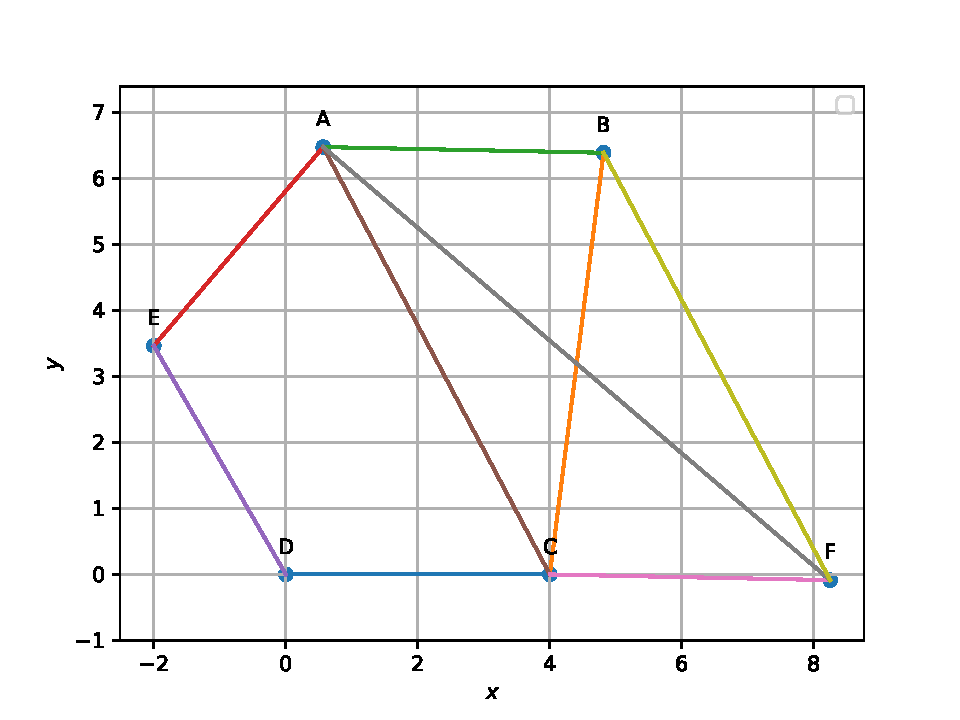
\includegraphics[width=\columnwidth]{chapters/9/9/3/11/figs/matrix.pdf}
		\caption{}
		\label{fig:9/9/3/11}
  	\end{figure}
	\begin{proof}
		Since $BF \parallel AC$,
		\begin{align}
			\vec{F}-\vec{B}&=k\brak{\vec{C}-\vec{A}}
			\\
			\implies \vec{F}&=\vec{B}+k\brak{\vec{C}-\vec{A}}
		\label{eq:9/9/3/11/f}
		\end{align}
		Thus, from  Appendix
  \ref{prop:area2d},
\begin{align}
ar (ACF)
	&= 
 \frac{1}{2}\norm{\vec{F} \times \vec{A}+\vec{A} \times \vec{C}+\vec{C} \times \vec{F}}
%ar (ACB)
% = 
% \frac{1}{2}\norm{\vec{A} \times \vec{B}+\vec{B} \times \vec{C}+\vec{C} \times \vec{A}}
		\label{eq:9/9/3/11/acf}
\end{align}
	Substituting from 
		\eqref{eq:9/9/3/11/f}
		in 
		\eqref{eq:9/9/3/11/acf},
\begin{align}
ar (ACF)
	&= \frac{1}{2}\norm{\cbrak{\vec{B}+k\brak{\vec{C}-\vec{A}}} \times \vec{A}+\vec{A} \times \vec{C}+\vec{C} \times \cbrak{\vec{B}+k\brak{\vec{C}-\vec{A}}}}
	\\
	&= \frac{1}{2}\norm{\vec{B} \times \vec{A}+\vec{A} \times \vec{C}+\vec{C} \times \vec{B}}
	\\
	&= ar\brak{ACB}
\end{align}
upon substituting from		from  Appendix
  \ref{prop:area2d}.
		\eqref{eq:9/9/3/11/pent}
		follows from 
		\eqref{eq:9/9/3/11}.

	\end{proof}

\iffalse

	    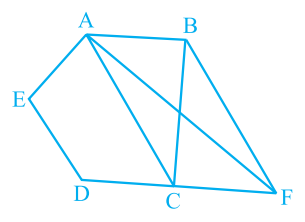
\includegraphics[scale=1.0]{diag_1.png}
   \section{Solution}
The input parameters for this construction are 
\begin{center}
\begin{tabular}{|c|c|c|}
	\hline
	\textbf{Symbol}&\textbf{Value}&\textbf{Description}\\
	\hline
	$\vec{D}$ & $\myvec{0\\0}$ & Point D\\
	\hline
	r1&4&DC\\
	\hline
	r2&8&DB\\
	\hline
	r3&6.5&DA\\
	\hline
	r4&4&DE\\
	\hline
	${\theta}_1$& 17$\pi/36$&$ \angle $BDC\\ 
	\hline
	${\theta}_2$& 53$\pi/180$&$ \angle $ADC\\ 
	\hline
	${\theta}_3$& 2$\pi/3$&$ \angle $EDC\\ 
	\hline
\end{tabular}
\end{center}
\begin{center}
Below python code realizes the above construction :
\fbox{\parbox{8.5cm}{\url{https://github.com/velicharlagokulkumar/FWC_module1/blob/main/matrices/lines/codes/matrix.py}}}
\end{center}
\textbf{termux commands :}
\begin{lstlisting}
bash sh.sh.........using shell command
\end{lstlisting}

\textbf{To Prove:} Ar($\vec{A}\vec{C}\vec{B}$)=Ar($\vec{A}\vec{C}\vec{F}$)
\begin{align}
\vec{F}=\vec{C}-\vec{A}+\vec{B}\end{align}
letting
\begin{align}
\vec{v1}=\vec{C}-\vec{A}\\ \vec{v2}=\vec{C}-\vec{F}
\end{align}
Area of the $\Delta \vec{A}\vec{C}\vec{F}$ is given by
\begin{align}
\frac{1}{2} \norm{\vec{v1}\times\vec{v2}}
\end{align}
letting
\begin{align}\vec{v3}=\vec{A}-\vec{C}\\ 
\vec{v4}=\vec{A}-\vec{B}
\end{align}
Area of the $\Delta \vec{A}\vec{C}\vec{B}$ is given by
\begin{align}
\frac{1}{2} \norm{\vec{v3}\times\vec{v4}}
\end{align}
\textbf{To Prove:}  Ar($\vec{A}\vec{E}\vec{D}\vec{F}$)=Ar($\vec{A}\vec{B}\vec{C}\vec{D}\vec{E}$) \\
Area of the $\Delta \vec{A}\vec{E}\vec{D}$ is given by
\begin{align}
\frac{1}{2} \norm{\vec{A}\times\vec{E}}
\end{align}
Area of the $\Delta \vec{A}\vec{D}\vec{C}$ is given by
\begin{align}
\frac{1}{2} \norm{\vec{A}\times\vec{C}}
\end{align}
From (8),(9)
\begin{center}
  Ar($\vec{A}\vec{E}\vec{D}\vec{C}$)=Ar($\Delta$$\vec{A}\vec{E}\vec{D}$)+Ar($\Delta$$\vec{A}\vec{D}\vec{C}$)     \ \ \ \ \ \ \ \ \ \  \ \ \ \ \ \ \ \ \ (10)   
\end{center}
 From (10),(4)
 \begin{center}
$\therefore$ Ar($\vec{A}\vec{E}\vec{D}\vec{F}$)=Ar($\vec{A}\vec{E}\vec{D}\vec{C}$)+Ar($\Delta$$\vec{A}\vec{C}\vec{F}$)
\end{center}
 From (10),(7)
 \begin{center}
$\therefore$ Ar($\vec{A}\vec{B}\vec{C}\vec{D}\vec{E}$)=Ar($\vec{A}\vec{E}\vec{D}\vec{C}$)+Ar($\Delta$$\vec{A}\vec{C}\vec{B}$)
\end{center}
 \section{Construction}
 	\begin{center}
  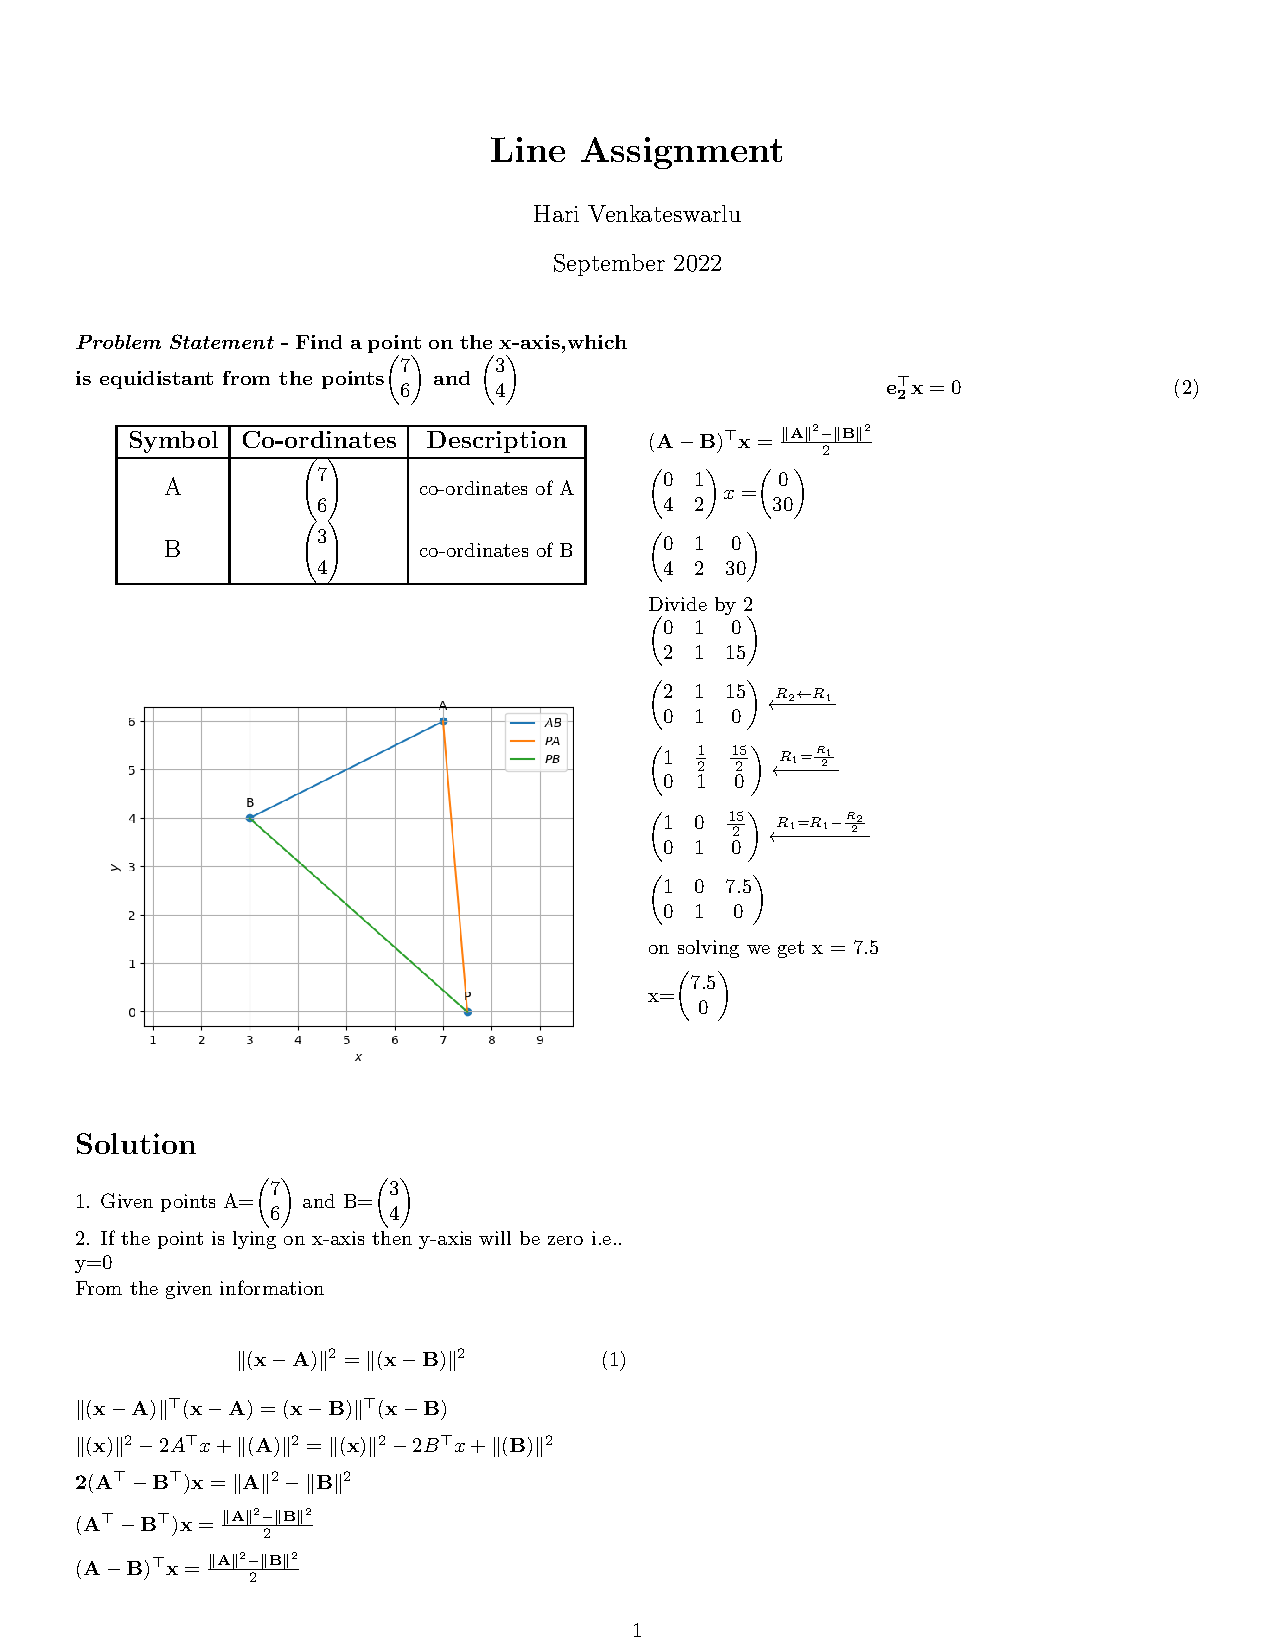
\includegraphics[scale=0.39]{matrix.pdf}\\
       Figure of construction 
  	\end{center}
\end{document}
\fi

\item 
\item 
\item 
\item 
\item 
\label{chapters/9/9/3/16}
\iffalse
\documentclass[a4paper,10pt]{report}
\usepackage[latin1]{inputenc}
\usepackage{amsmath}
\usepackage{amsmath,bm}
\usepackage{amsthm}
\usepackage{mathtools}
\usepackage{amsfonts}
\usepackage{amssymb}
\usepackage{graphicx}
\usepackage{array}
\usepackage{booktabs}
\usepackage{hyperref}
\usepackage{multicol}
\usepackage[margin=0.5in]{geometry}
\usepackage{karnaugh-map}
\usepackage[framemethod=tikz]{mdframed}
\newcommand{\myvec}[1]{ensuremat{\begin{pmatrix}#1\end{pmatrix}}}
	\let\vec\mathbf
\begin{document}

\raggedright{
\includegraphics[width=0.75\columnwidth]{logo.png}}\hspace{12.425cm}\raggedleft FWC22037\vspace{2mm}
\\
\centering\Large\textbf{ASSIGNMENT-MATRICES}\vspace{5mm}


\begin{multicols}{2}
\centering \large\textsc{C}\footnotesize\textsc{ontents}\vspace{5mm}
\\
\raggedright\large\textbf{1.\hspace{1cm}Problem}\hspace{3cm}1\vspace{5mm}\\
\raggedright\large\textbf{2.\hspace{1cm}Solution}\hspace{3.1cm}1\vspace{5mm}\\
\raggedright\large\textbf{3.\hspace{1cm}Construction}\hspace{2.1cm}1\vspace{5mm}\\


\centering \large\textsc{1.  P}\footnotesize\textsc{ROBLEM}\vspace{5mm}\\
\fi
In the Figure 
		\ref{fig:9/9/3/16},
	\begin{figure}[H]
		\centering
 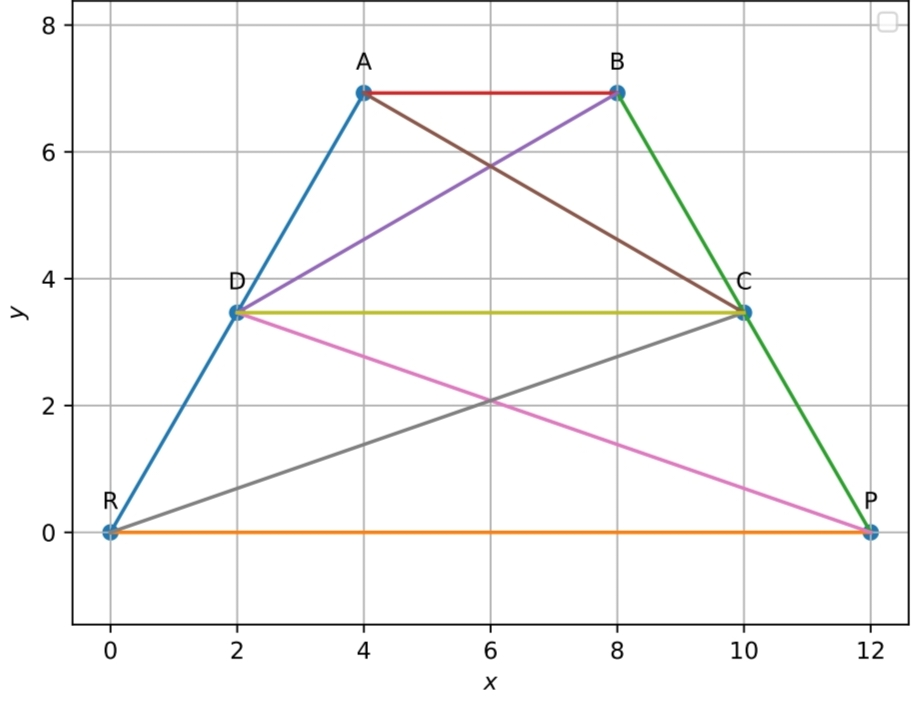
\includegraphics[width=0.75\columnwidth]{chapters/9/9/3/16/figs/main.jpg}
		\caption{}
		\label{fig:9/9/3/16}
  	\end{figure}
	\begin{align}
		\label{eq:9/9/3/16}
		ar(DRC) &= ar(DPC)
		\\
		ar(BDP) &= ar(ARC).
\end{align}
 Show that the quadrilaterals $ABCD$ and $DCPR$ are trapeziums.
\begin{proof}
From Appendix
  \ref{prop:area2d-norm}
 and 
		\eqref{eq:9/9/3/16},
\begin{align}
	\frac{1}{2}\norm{\brak{\vec{D}-\vec{R}} \times \brak{\vec{D}-\vec{C}}}
	&=
	\frac{1}{2}\norm{\brak{\vec{C}-\vec{D}} \times \brak{\vec{C}-\vec{P}}}
	\\
	\implies
	\brak{\vec{D}-\vec{R}}\times \brak{\vec{D}-\vec{C}}  
	&=
	\brak{\vec{C}-\vec{D}} \times \brak{\vec{C}-\vec{P}}
  \end{align}
  which can be expressed as 
  \begin{align}
	\brak{\vec{C}-\vec{D}} \times \brak{\vec{C}-\vec{D}+\vec{R}-\vec{P}} &=\vec{0} 
	\\
\implies 
	\brak{\vec{C}-\vec{D}} \times \brak{\vec{R}-\vec{P}} &=\vec{0} 
	\\
	  \text{or, } CD \parallel RP
  \end{align}
  Hence, $DCPR$ is a trapezium.  Similarly, it can be shown that $ABCD$ is also a trapezium.

%	  \frac{1}{2}\brak{\vec{C}-\vec{D}}\brak{\frac{1}{2}\brak{\vec{D}-\vec{R}}\times \brak{\vec{D}-\vec{C}}  
%
%	&=
%	 \times \brak{\vec{C}-\vec{P}}
%  \end{align}

\end{proof}
  \iffalse

\centering \large\textsc{2.  S}\footnotesize\textsc{OLUTION}\vspace{5mm}\\ \raggedright\large 1. Given that the area of the triangles \textbf{DRC} and \textbf{DPC} are equal.\\
\raggedright \large 2. From triangles \textbf{DCR} and \textbf{DPC}
\begin{gather}
 \frac{1}{2} \vec{[(D-C)x(D-R)]} =  \frac{1}{2} \vec{[(C-D)x(C-P)
 ]}
\end{gather}
\begin{align*}
 \vec{(C-D) x [(C-P)-(D-R)]} = 0\\
 \vec{(C-D) x [C-P-D+R]} = 0 \\
 \vec{(C-D) x (C-D) + (C-D) x (R-P) = 0}
\end{align*} 
\begin{align}
\vec{(C-D) x (R-P) = 0}
\end{align}
\raggedright 3. From equation 2 the cross product is 0 the lines \textbf{A-B} is parallel to \textbf{D-C} and the quadrilateral \textbf{DCRP} a Trapezium.\\
\raggedright 4. Given that the area of the triangles \textbf{BDP} and \textbf{ARC} are equal. From the information given we can say the area of triangles \textbf{ADC} and \textbf{BCD}. 
\begin{gather}
\frac{1}{2} \vec{[(D-C)x(D-A)]} =  \frac{1}{2} \vec{[(C-D)x(C-B)]}
\end{gather}
\begin{align*}
 \vec{(C-D) x [(C-B)-(D-A)]} = 0\\
 \vec{(C-D) x [C-B-D+A]} = 0 \\
 \vec{(C-D) x (C-D) + (C-D) x (A-B) = 0}
\end{align*}
\begin{align}
\vec{(C-D) x (A-B) = 0}
\end{align}
\raggedright 5. From equation 4 the cross product is 0 the lines \textbf{A-B} is parallel to \textbf{D-C} and the quadrilateral \textbf{ABCD} a Trapezium.\\
\vspace{2mm}
\centering{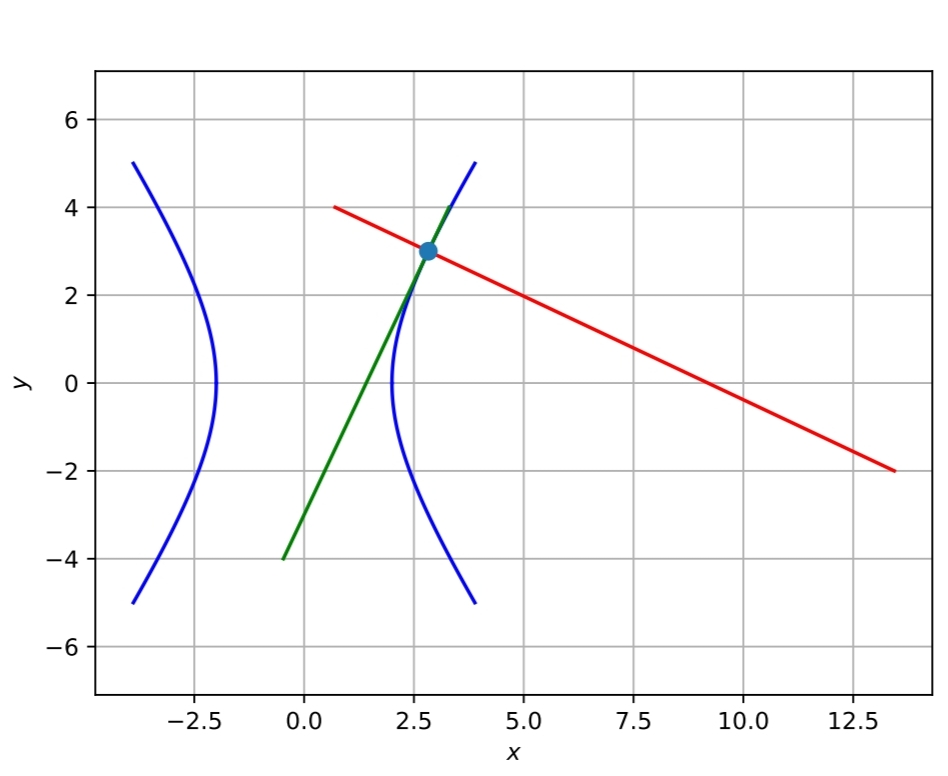
\includegraphics[width=0.75\columnwidth]{main.jpg}}\vspace{2mm}\\
\centering\normalsize{Figure}\vspace{5mm}\\


\centering \large\textsc{3.  C}\footnotesize\textsc{ONSTRUCTION}\vspace{5mm}\\
\begin{center}
    \label{tab:truthtable}
    \setlength{\arrayrulewidth}{0.2mm}
\setlength{\tabcolsep}{5pt}
\renewcommand{\arraystretch}{2}
    \begin{tabular}{|c|c|c|}
    \hline % <-- Alignments: 1st column left, 2nd middle and 3rd right, with vertical lines in between
      \large\textbf{Symbol} & \large\textbf{Co-ordinates} & \large\textbf{Description}\\
      \hline
	\large a & 12 & \large RP\\
	\large c & 8 & \large RA\\
	\large b & 4 & \large AB\\
	\large R &  $\ \begin{pmatrix} 0\\0 \end{pmatrix}$  & \large point vector R\\
	\large P &  $\ \begin{pmatrix} a\\0 \end{pmatrix}$ & \large point vector P\\
	\large A &  $\ \begin{pmatrix} c.cos(\theta) \\ c. sin(\theta) \end{pmatrix}$ & \large point vector A\\ 
		\large\textbf B & {A+P}  & \large point vector B\\ 
      \hline 
   \end{tabular}
 \end{center}\vspace{10mm} 


\raggedright\large{The figure above is generated using python code provided in the below source code link.}\vspace{2mm}\\
\begin{mdframed}
\raggedright\large{https://github.com/siva-gayathri \\ /FWC/blob/main/assigment-1/codes/main.py}
\end{mdframed}


\end{multicols}
\end{document}
\fi

\iffalse
\item 
\label{chapters/9/9/3/4}
\iffalse
\def\mytitle{MATRICES USING PYTHON}
\def\myauthor{P.kalyan}
\def\contact{kalyanpadyalaanirudh@gmail.com}
\def\mymodule{Future Wireless Communication (FWC)}
\documentclass[10pt, a4paper]{article}
\usepackage[a4paper,outer=1.5cm,inner=1.5cm,top=1.75cm,bottom=1.5cm]{geometry}
\twocolumn
\usepackage{graphicx}
\graphicspath{{./images/}}
\usepackage[colorlinks,linkcolor={black},citecolor={blue!80!black},urlcolor={blue!80!black}]{hyperref}
\usepackage[parfill]{parskip}
\usepackage{lmodern}
\usepackage{tikz}
	\usepackage{physics}
%\documentclass[tikz, border=2mm]{standalone}
\usepackage{karnaugh-map}
%\documentclass{article}
\usepackage{tabularx}
\usepackage{circuitikz}
\usetikzlibrary{calc}
\usepackage{amsmath}
\usepackage{amssymb}
\renewcommand*\familydefault{\sfdefault}
\usepackage{watermark}
\usepackage{lipsum}
\usepackage{xcolor}
\usepackage{listings}
\usepackage{float}
\usepackage{titlesec}
\providecommand{\mtx}[1]{\mathbf{#1}}
\titlespacing{\subsection}{1pt}{\parskip}{3pt}
\titlespacing{\subsubsection}{0pt}{\parskip}{-\parskip}
\titlespacing{\paragraph}{0pt}{\parskip}{\parskip}
\newcommand{\figuremacro}[5]{
    \begin{figure}[H]
        \centering
        \includegraphics[width=0.75\columnwidth]{#2}
        \caption[#3]{\textbf{#3}#4}
        \label{fig:#2}
    \end{figure}
}
\newcommand{\myvec}[1]{\ensuremath{\begin{pmatrix}#1\end{pmatrix}}}
\let\vec\mathbf
\lstset{
frame=single, 
breaklines=true,
columns=fullflexible
}

\thiswatermark{\centering \put(0,-90){
\includegraphics[width=0.75\columnwidth]{iith}} }
\title{\mytitle}
\author{\myauthor\hspace{1em}\\\contact\\FWC22031\hspace{6.5em}IITH\hspace{0.5em}\mymodule\hspace{6em}ASSIGN-5}
\date{}
\begin{document}
	\maketitle
	\tableofcontents
   \section{Problem}
   \fi
   $ABC, ABD$ are 2 triangles on same base $AB$, if line segment $CD$ is bisected by $AB$ at $\vec{O}$, show that 
   \begin{align}
		\label{eq:9/9/3/4}
 ar (ABC) = ar (ABD)  
   \end{align}
	\begin{figure}[H]
		\centering
 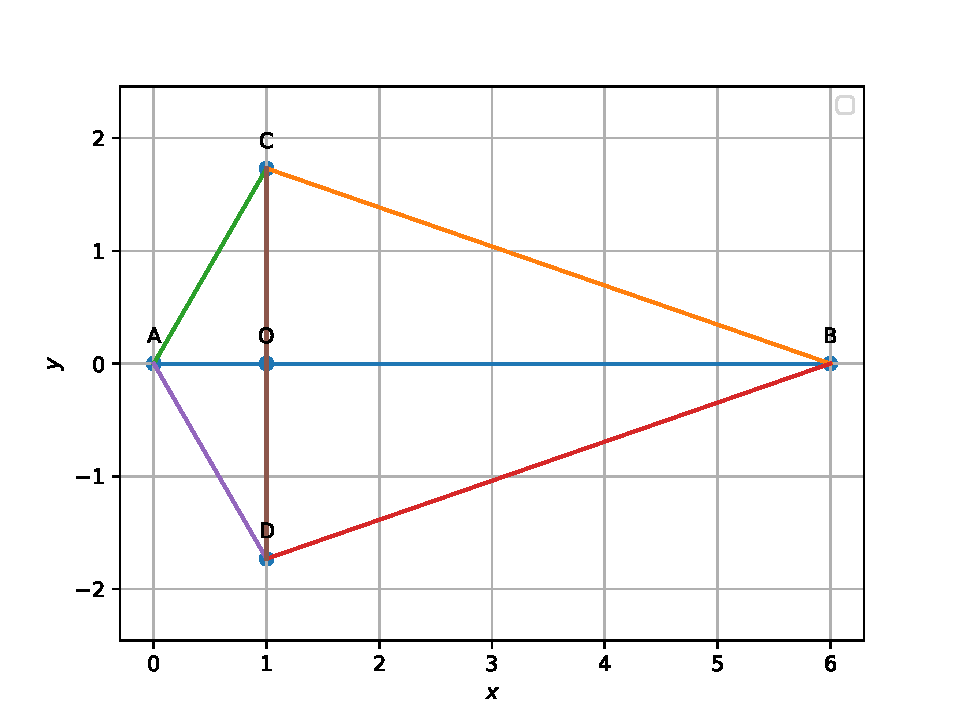
\includegraphics[width=0.75\columnwidth]{chapters/9/9/3/4/figs/figa6.pdf}
		\caption{}
		\label{fig:9/9/3/4}
  	\end{figure}
	\begin{proof}
		See Fig. 
		\ref{fig:9/9/3/4}. $AO$ and $OB$ are medians of triangles $ADC$ and $BDC$. From 
Appendix	  \ref{prop:two-median-area}, 
		\eqref{eq:9/9/3/4} is trivial.
	\end{proof}


\iffalse

	    \includegraphics[width=0.75\columnwidth]{}
   \section{Solution}
   \textbf{Theory:}\\
In 2 triangles with same base and linesegment cd is bisected at o  
\textbf{To Prove:} Ar(ABC)=Ar(ABD) \\
\textbf{Theorem} : Two triangles on the same base (or equal bases) and having the equal heights are equal in area.
\begin{center}
$\therefore$ Ar($\Delta$ ABC)=Ar($\Delta$ ABD)......(1)\\
Hence, Proved    
\end{center}


\
\textbf{termux commands :}
\begin{lstlisting}
python3 matrix.py
\end{lstlisting}


The input parameters for this construction are 
\begin{center}
\begin{tabular}{|c|c|c|}
	\hline
	\textbf{Symbol}&\textbf{Value}&\textbf{Description}\\
	\hline
	k1&4&length of CD\\
	\hline
	k2&6&length of AB\\
	\hline
 
	\hline
	O&$\
	\begin{pmatrix}
		0 \\
		0 \\
	\end{pmatrix}$%
	&Point O\\
	
	\hline
\end{tabular}
\end{center}
\textbf{To Prove:} Ar(ABC)=Ar(ABD)
  %	\begin{align}
	%		\vec{C} &= \myvec{0 \\ 0}, \vec{E}=\myvec{-5 \\ 3}\\
	%			\vec{F} &= \myvec{3 \\ 0}, \vec{D}=\myvec{-3 \\ 0}
	%	\end{align}
		\begin{center}
	a=A-B\\
	b=C-B\\
	c=B-D\\
	Area of the $\Delta$ABC is given by \\
Ar($\Delta$ABC) =$\frac{1}{2}$$\norm{\vec{a}\times\vec{b}}$............(2)\\
    b=C-B\\
	c=B-D\\
		Area of the $\Delta$ABD is given by \\
 Ar($\Delta$ABD) =$\frac{1}{2}$$\norm{\vec{c}\times\vec{d}}$...............(3)
	\end{center}
	
	\begin{center}
$\therefore$ Ar(ABC)=Ar(ABD)........(4)\\
	\end{center}
The below python code realizes the above construction:	
\begin{lstlisting}
https://github.com/anirudhkalyan/fwc
\end{lstlisting}
 \section{Construction}
 	\begin{center}
  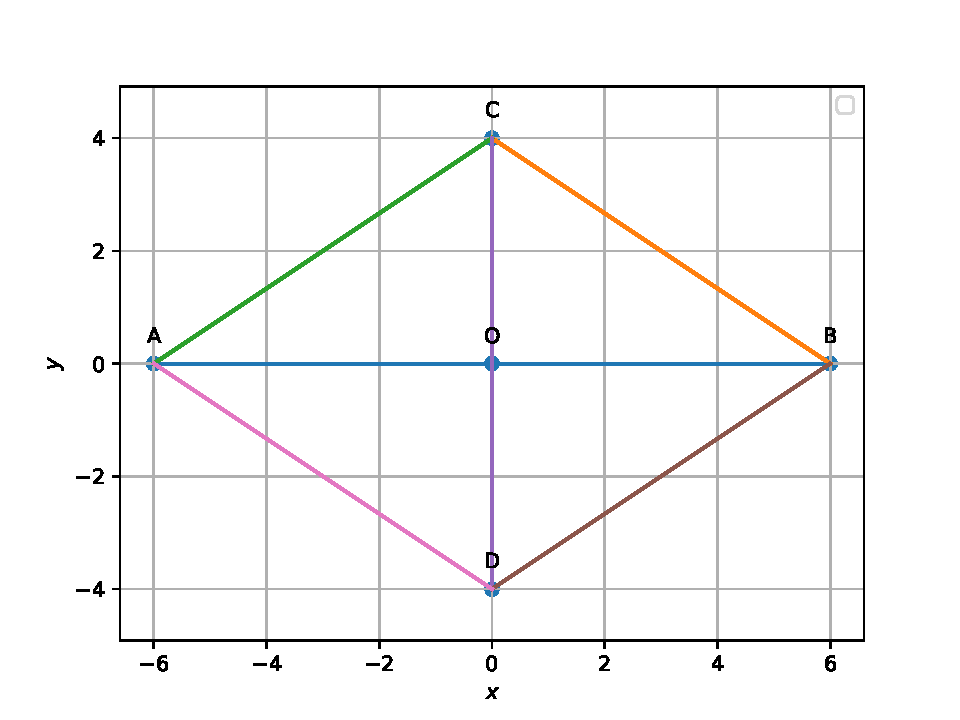
\includegraphics[width=0.75\columnwidth]{figsa1.pdf}
  
  Figure of construction
  	\end{center}
  	  
\bibliographystyle{ieeetr}
\end{document}
\fi

\item 
\label{chapters/9/9/3/4}
\iffalse
\def\mytitle{MATRICES USING PYTHON}
\def\myauthor{P.kalyan}
\def\contact{kalyanpadyalaanirudh@gmail.com}
\def\mymodule{Future Wireless Communication (FWC)}
\documentclass[10pt, a4paper]{article}
\usepackage[a4paper,outer=1.5cm,inner=1.5cm,top=1.75cm,bottom=1.5cm]{geometry}
\twocolumn
\usepackage{graphicx}
\graphicspath{{./images/}}
\usepackage[colorlinks,linkcolor={black},citecolor={blue!80!black},urlcolor={blue!80!black}]{hyperref}
\usepackage[parfill]{parskip}
\usepackage{lmodern}
\usepackage{tikz}
	\usepackage{physics}
%\documentclass[tikz, border=2mm]{standalone}
\usepackage{karnaugh-map}
%\documentclass{article}
\usepackage{tabularx}
\usepackage{circuitikz}
\usetikzlibrary{calc}
\usepackage{amsmath}
\usepackage{amssymb}
\renewcommand*\familydefault{\sfdefault}
\usepackage{watermark}
\usepackage{lipsum}
\usepackage{xcolor}
\usepackage{listings}
\usepackage{float}
\usepackage{titlesec}
\providecommand{\mtx}[1]{\mathbf{#1}}
\titlespacing{\subsection}{1pt}{\parskip}{3pt}
\titlespacing{\subsubsection}{0pt}{\parskip}{-\parskip}
\titlespacing{\paragraph}{0pt}{\parskip}{\parskip}
\newcommand{\figuremacro}[5]{
    \begin{figure}[H]
        \centering
        \includegraphics[width=0.75\columnwidth]{#2}
        \caption[#3]{\textbf{#3}#4}
        \label{fig:#2}
    \end{figure}
}
\newcommand{\myvec}[1]{\ensuremath{\begin{pmatrix}#1\end{pmatrix}}}
\let\vec\mathbf
\lstset{
frame=single, 
breaklines=true,
columns=fullflexible
}

\thiswatermark{\centering \put(0,-90){
\includegraphics[width=0.75\columnwidth]{iith}} }
\title{\mytitle}
\author{\myauthor\hspace{1em}\\\contact\\FWC22031\hspace{6.5em}IITH\hspace{0.5em}\mymodule\hspace{6em}ASSIGN-5}
\date{}
\begin{document}
	\maketitle
	\tableofcontents
   \section{Problem}
   \fi
   $ABC, ABD$ are 2 triangles on same base $AB$, if line segment $CD$ is bisected by $AB$ at $\vec{O}$, show that 
   \begin{align}
		\label{eq:9/9/3/4}
 ar (ABC) = ar (ABD)  
   \end{align}
	\begin{figure}[H]
		\centering
 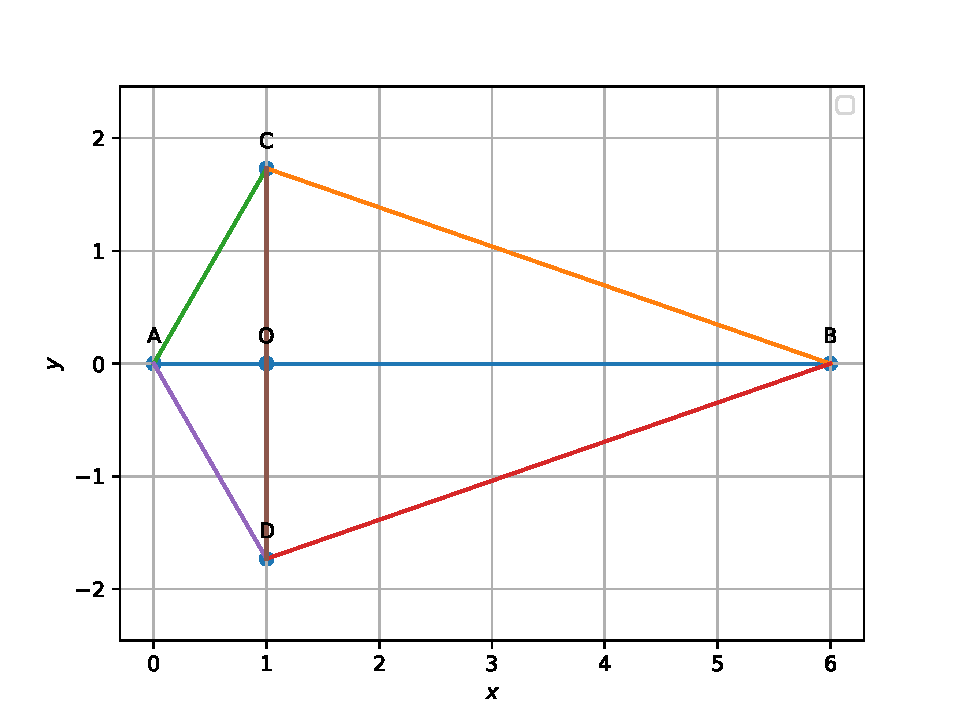
\includegraphics[width=0.75\columnwidth]{chapters/9/9/3/4/figs/figa6.pdf}
		\caption{}
		\label{fig:9/9/3/4}
  	\end{figure}
	\begin{proof}
		See Fig. 
		\ref{fig:9/9/3/4}. $AO$ and $OB$ are medians of triangles $ADC$ and $BDC$. From 
Appendix	  \ref{prop:two-median-area}, 
		\eqref{eq:9/9/3/4} is trivial.
	\end{proof}


\iffalse

	    \includegraphics[width=0.75\columnwidth]{}
   \section{Solution}
   \textbf{Theory:}\\
In 2 triangles with same base and linesegment cd is bisected at o  
\textbf{To Prove:} Ar(ABC)=Ar(ABD) \\
\textbf{Theorem} : Two triangles on the same base (or equal bases) and having the equal heights are equal in area.
\begin{center}
$\therefore$ Ar($\Delta$ ABC)=Ar($\Delta$ ABD)......(1)\\
Hence, Proved    
\end{center}


\
\textbf{termux commands :}
\begin{lstlisting}
python3 matrix.py
\end{lstlisting}


The input parameters for this construction are 
\begin{center}
\begin{tabular}{|c|c|c|}
	\hline
	\textbf{Symbol}&\textbf{Value}&\textbf{Description}\\
	\hline
	k1&4&length of CD\\
	\hline
	k2&6&length of AB\\
	\hline
 
	\hline
	O&$\
	\begin{pmatrix}
		0 \\
		0 \\
	\end{pmatrix}$%
	&Point O\\
	
	\hline
\end{tabular}
\end{center}
\textbf{To Prove:} Ar(ABC)=Ar(ABD)
  %	\begin{align}
	%		\vec{C} &= \myvec{0 \\ 0}, \vec{E}=\myvec{-5 \\ 3}\\
	%			\vec{F} &= \myvec{3 \\ 0}, \vec{D}=\myvec{-3 \\ 0}
	%	\end{align}
		\begin{center}
	a=A-B\\
	b=C-B\\
	c=B-D\\
	Area of the $\Delta$ABC is given by \\
Ar($\Delta$ABC) =$\frac{1}{2}$$\norm{\vec{a}\times\vec{b}}$............(2)\\
    b=C-B\\
	c=B-D\\
		Area of the $\Delta$ABD is given by \\
 Ar($\Delta$ABD) =$\frac{1}{2}$$\norm{\vec{c}\times\vec{d}}$...............(3)
	\end{center}
	
	\begin{center}
$\therefore$ Ar(ABC)=Ar(ABD)........(4)\\
	\end{center}
The below python code realizes the above construction:	
\begin{lstlisting}
https://github.com/anirudhkalyan/fwc
\end{lstlisting}
 \section{Construction}
 	\begin{center}
  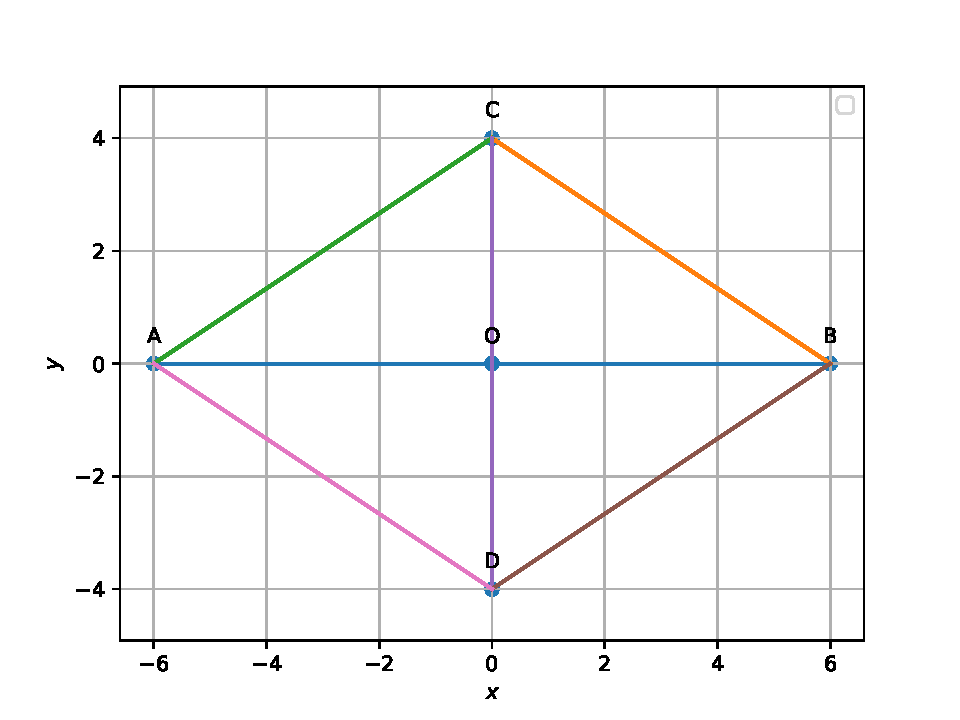
\includegraphics[width=0.75\columnwidth]{figsa1.pdf}
  
  Figure of construction
  	\end{center}
  	  
\bibliographystyle{ieeetr}
\end{document}
\fi

\item 
\label{chapters/9/9/3/4}
\iffalse
\def\mytitle{MATRICES USING PYTHON}
\def\myauthor{P.kalyan}
\def\contact{kalyanpadyalaanirudh@gmail.com}
\def\mymodule{Future Wireless Communication (FWC)}
\documentclass[10pt, a4paper]{article}
\usepackage[a4paper,outer=1.5cm,inner=1.5cm,top=1.75cm,bottom=1.5cm]{geometry}
\twocolumn
\usepackage{graphicx}
\graphicspath{{./images/}}
\usepackage[colorlinks,linkcolor={black},citecolor={blue!80!black},urlcolor={blue!80!black}]{hyperref}
\usepackage[parfill]{parskip}
\usepackage{lmodern}
\usepackage{tikz}
	\usepackage{physics}
%\documentclass[tikz, border=2mm]{standalone}
\usepackage{karnaugh-map}
%\documentclass{article}
\usepackage{tabularx}
\usepackage{circuitikz}
\usetikzlibrary{calc}
\usepackage{amsmath}
\usepackage{amssymb}
\renewcommand*\familydefault{\sfdefault}
\usepackage{watermark}
\usepackage{lipsum}
\usepackage{xcolor}
\usepackage{listings}
\usepackage{float}
\usepackage{titlesec}
\providecommand{\mtx}[1]{\mathbf{#1}}
\titlespacing{\subsection}{1pt}{\parskip}{3pt}
\titlespacing{\subsubsection}{0pt}{\parskip}{-\parskip}
\titlespacing{\paragraph}{0pt}{\parskip}{\parskip}
\newcommand{\figuremacro}[5]{
    \begin{figure}[H]
        \centering
        \includegraphics[width=0.75\columnwidth]{#2}
        \caption[#3]{\textbf{#3}#4}
        \label{fig:#2}
    \end{figure}
}
\newcommand{\myvec}[1]{\ensuremath{\begin{pmatrix}#1\end{pmatrix}}}
\let\vec\mathbf
\lstset{
frame=single, 
breaklines=true,
columns=fullflexible
}

\thiswatermark{\centering \put(0,-90){
\includegraphics[width=0.75\columnwidth]{iith}} }
\title{\mytitle}
\author{\myauthor\hspace{1em}\\\contact\\FWC22031\hspace{6.5em}IITH\hspace{0.5em}\mymodule\hspace{6em}ASSIGN-5}
\date{}
\begin{document}
	\maketitle
	\tableofcontents
   \section{Problem}
   \fi
   $ABC, ABD$ are 2 triangles on same base $AB$, if line segment $CD$ is bisected by $AB$ at $\vec{O}$, show that 
   \begin{align}
		\label{eq:9/9/3/4}
 ar (ABC) = ar (ABD)  
   \end{align}
	\begin{figure}[H]
		\centering
 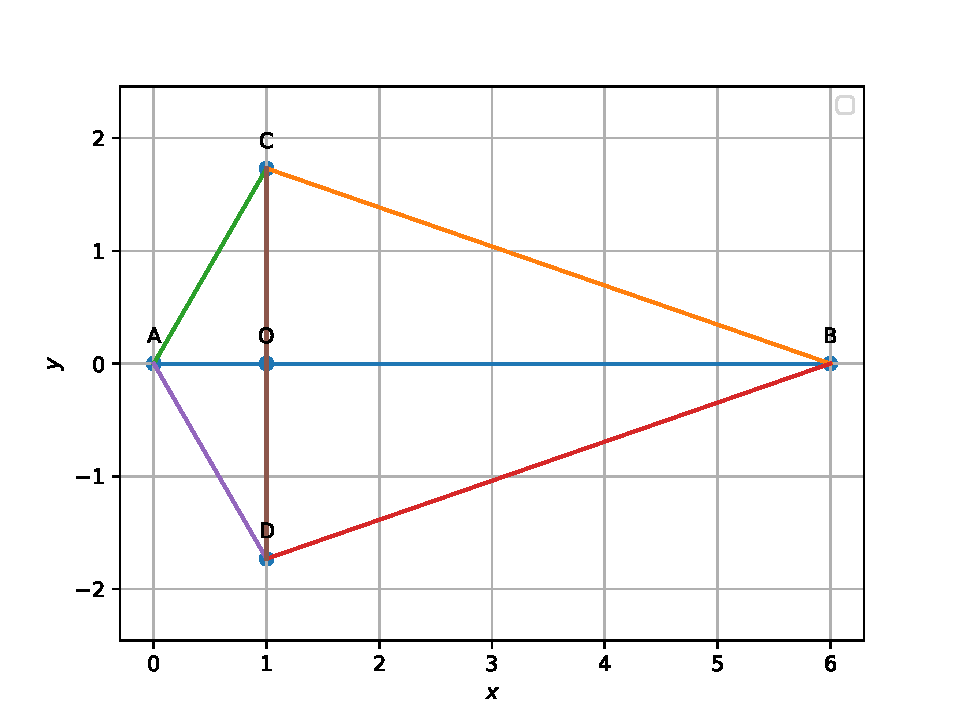
\includegraphics[width=0.75\columnwidth]{chapters/9/9/3/4/figs/figa6.pdf}
		\caption{}
		\label{fig:9/9/3/4}
  	\end{figure}
	\begin{proof}
		See Fig. 
		\ref{fig:9/9/3/4}. $AO$ and $OB$ are medians of triangles $ADC$ and $BDC$. From 
Appendix	  \ref{prop:two-median-area}, 
		\eqref{eq:9/9/3/4} is trivial.
	\end{proof}


\iffalse

	    \includegraphics[width=0.75\columnwidth]{}
   \section{Solution}
   \textbf{Theory:}\\
In 2 triangles with same base and linesegment cd is bisected at o  
\textbf{To Prove:} Ar(ABC)=Ar(ABD) \\
\textbf{Theorem} : Two triangles on the same base (or equal bases) and having the equal heights are equal in area.
\begin{center}
$\therefore$ Ar($\Delta$ ABC)=Ar($\Delta$ ABD)......(1)\\
Hence, Proved    
\end{center}


\
\textbf{termux commands :}
\begin{lstlisting}
python3 matrix.py
\end{lstlisting}


The input parameters for this construction are 
\begin{center}
\begin{tabular}{|c|c|c|}
	\hline
	\textbf{Symbol}&\textbf{Value}&\textbf{Description}\\
	\hline
	k1&4&length of CD\\
	\hline
	k2&6&length of AB\\
	\hline
 
	\hline
	O&$\
	\begin{pmatrix}
		0 \\
		0 \\
	\end{pmatrix}$%
	&Point O\\
	
	\hline
\end{tabular}
\end{center}
\textbf{To Prove:} Ar(ABC)=Ar(ABD)
  %	\begin{align}
	%		\vec{C} &= \myvec{0 \\ 0}, \vec{E}=\myvec{-5 \\ 3}\\
	%			\vec{F} &= \myvec{3 \\ 0}, \vec{D}=\myvec{-3 \\ 0}
	%	\end{align}
		\begin{center}
	a=A-B\\
	b=C-B\\
	c=B-D\\
	Area of the $\Delta$ABC is given by \\
Ar($\Delta$ABC) =$\frac{1}{2}$$\norm{\vec{a}\times\vec{b}}$............(2)\\
    b=C-B\\
	c=B-D\\
		Area of the $\Delta$ABD is given by \\
 Ar($\Delta$ABD) =$\frac{1}{2}$$\norm{\vec{c}\times\vec{d}}$...............(3)
	\end{center}
	
	\begin{center}
$\therefore$ Ar(ABC)=Ar(ABD)........(4)\\
	\end{center}
The below python code realizes the above construction:	
\begin{lstlisting}
https://github.com/anirudhkalyan/fwc
\end{lstlisting}
 \section{Construction}
 	\begin{center}
  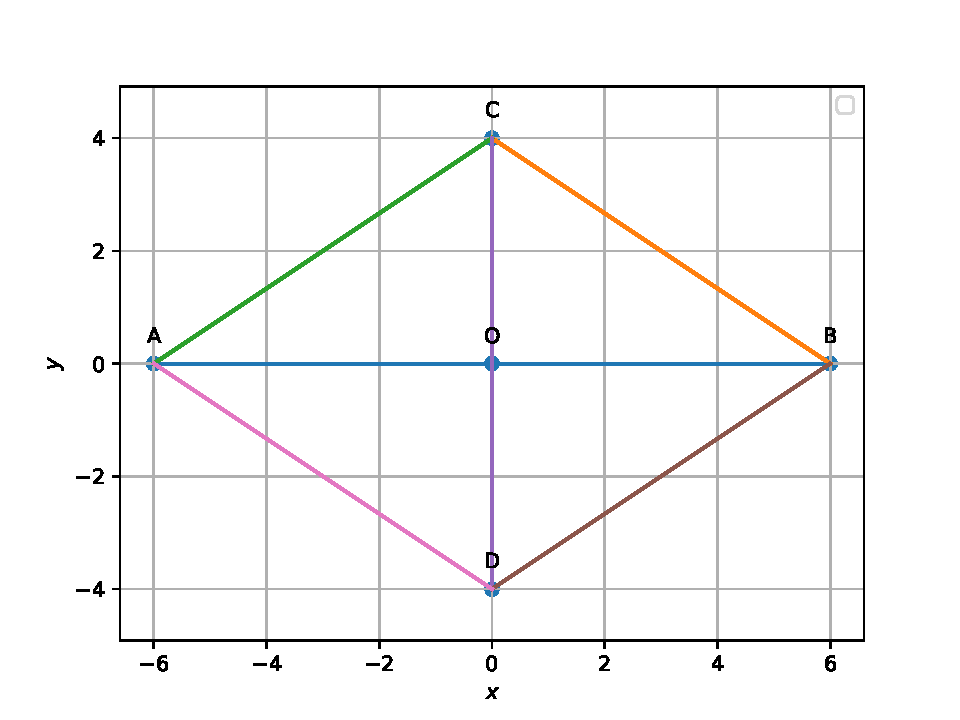
\includegraphics[width=0.75\columnwidth]{figsa1.pdf}
  
  Figure of construction
  	\end{center}
  	  
\bibliographystyle{ieeetr}
\end{document}
\fi

\item 
\label{chapters/9/9/3/4}
\iffalse
\def\mytitle{MATRICES USING PYTHON}
\def\myauthor{P.kalyan}
\def\contact{kalyanpadyalaanirudh@gmail.com}
\def\mymodule{Future Wireless Communication (FWC)}
\documentclass[10pt, a4paper]{article}
\usepackage[a4paper,outer=1.5cm,inner=1.5cm,top=1.75cm,bottom=1.5cm]{geometry}
\twocolumn
\usepackage{graphicx}
\graphicspath{{./images/}}
\usepackage[colorlinks,linkcolor={black},citecolor={blue!80!black},urlcolor={blue!80!black}]{hyperref}
\usepackage[parfill]{parskip}
\usepackage{lmodern}
\usepackage{tikz}
	\usepackage{physics}
%\documentclass[tikz, border=2mm]{standalone}
\usepackage{karnaugh-map}
%\documentclass{article}
\usepackage{tabularx}
\usepackage{circuitikz}
\usetikzlibrary{calc}
\usepackage{amsmath}
\usepackage{amssymb}
\renewcommand*\familydefault{\sfdefault}
\usepackage{watermark}
\usepackage{lipsum}
\usepackage{xcolor}
\usepackage{listings}
\usepackage{float}
\usepackage{titlesec}
\providecommand{\mtx}[1]{\mathbf{#1}}
\titlespacing{\subsection}{1pt}{\parskip}{3pt}
\titlespacing{\subsubsection}{0pt}{\parskip}{-\parskip}
\titlespacing{\paragraph}{0pt}{\parskip}{\parskip}
\newcommand{\figuremacro}[5]{
    \begin{figure}[H]
        \centering
        \includegraphics[width=0.75\columnwidth]{#2}
        \caption[#3]{\textbf{#3}#4}
        \label{fig:#2}
    \end{figure}
}
\newcommand{\myvec}[1]{\ensuremath{\begin{pmatrix}#1\end{pmatrix}}}
\let\vec\mathbf
\lstset{
frame=single, 
breaklines=true,
columns=fullflexible
}

\thiswatermark{\centering \put(0,-90){
\includegraphics[width=0.75\columnwidth]{iith}} }
\title{\mytitle}
\author{\myauthor\hspace{1em}\\\contact\\FWC22031\hspace{6.5em}IITH\hspace{0.5em}\mymodule\hspace{6em}ASSIGN-5}
\date{}
\begin{document}
	\maketitle
	\tableofcontents
   \section{Problem}
   \fi
   $ABC, ABD$ are 2 triangles on same base $AB$, if line segment $CD$ is bisected by $AB$ at $\vec{O}$, show that 
   \begin{align}
		\label{eq:9/9/3/4}
 ar (ABC) = ar (ABD)  
   \end{align}
	\begin{figure}[H]
		\centering
 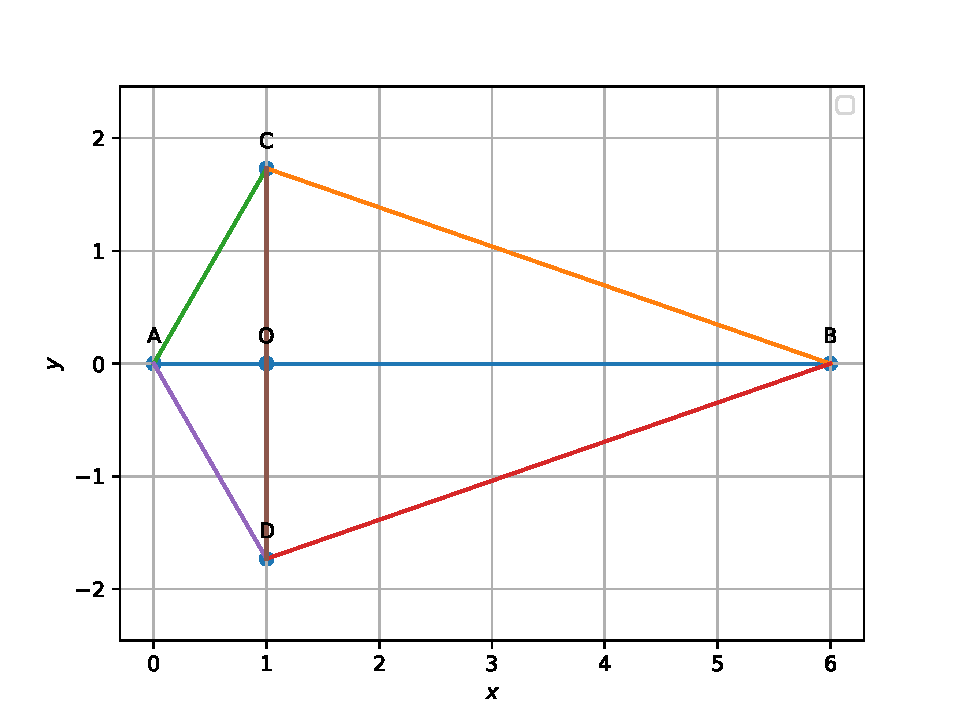
\includegraphics[width=0.75\columnwidth]{chapters/9/9/3/4/figs/figa6.pdf}
		\caption{}
		\label{fig:9/9/3/4}
  	\end{figure}
	\begin{proof}
		See Fig. 
		\ref{fig:9/9/3/4}. $AO$ and $OB$ are medians of triangles $ADC$ and $BDC$. From 
Appendix	  \ref{prop:two-median-area}, 
		\eqref{eq:9/9/3/4} is trivial.
	\end{proof}


\iffalse

	    \includegraphics[width=0.75\columnwidth]{}
   \section{Solution}
   \textbf{Theory:}\\
In 2 triangles with same base and linesegment cd is bisected at o  
\textbf{To Prove:} Ar(ABC)=Ar(ABD) \\
\textbf{Theorem} : Two triangles on the same base (or equal bases) and having the equal heights are equal in area.
\begin{center}
$\therefore$ Ar($\Delta$ ABC)=Ar($\Delta$ ABD)......(1)\\
Hence, Proved    
\end{center}


\
\textbf{termux commands :}
\begin{lstlisting}
python3 matrix.py
\end{lstlisting}


The input parameters for this construction are 
\begin{center}
\begin{tabular}{|c|c|c|}
	\hline
	\textbf{Symbol}&\textbf{Value}&\textbf{Description}\\
	\hline
	k1&4&length of CD\\
	\hline
	k2&6&length of AB\\
	\hline
 
	\hline
	O&$\
	\begin{pmatrix}
		0 \\
		0 \\
	\end{pmatrix}$%
	&Point O\\
	
	\hline
\end{tabular}
\end{center}
\textbf{To Prove:} Ar(ABC)=Ar(ABD)
  %	\begin{align}
	%		\vec{C} &= \myvec{0 \\ 0}, \vec{E}=\myvec{-5 \\ 3}\\
	%			\vec{F} &= \myvec{3 \\ 0}, \vec{D}=\myvec{-3 \\ 0}
	%	\end{align}
		\begin{center}
	a=A-B\\
	b=C-B\\
	c=B-D\\
	Area of the $\Delta$ABC is given by \\
Ar($\Delta$ABC) =$\frac{1}{2}$$\norm{\vec{a}\times\vec{b}}$............(2)\\
    b=C-B\\
	c=B-D\\
		Area of the $\Delta$ABD is given by \\
 Ar($\Delta$ABD) =$\frac{1}{2}$$\norm{\vec{c}\times\vec{d}}$...............(3)
	\end{center}
	
	\begin{center}
$\therefore$ Ar(ABC)=Ar(ABD)........(4)\\
	\end{center}
The below python code realizes the above construction:	
\begin{lstlisting}
https://github.com/anirudhkalyan/fwc
\end{lstlisting}
 \section{Construction}
 	\begin{center}
  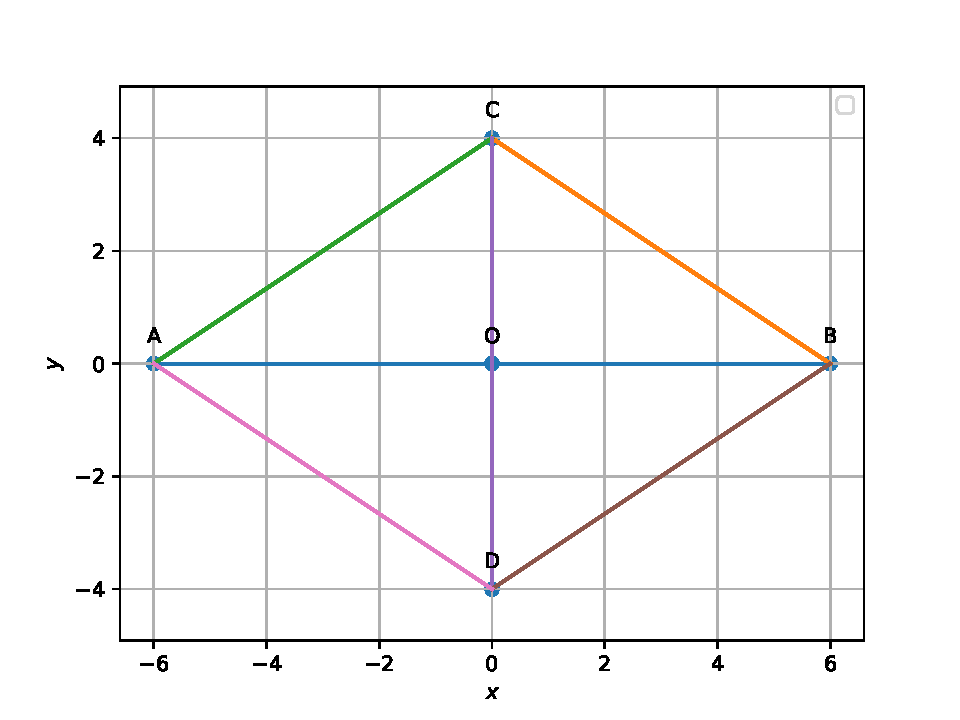
\includegraphics[width=0.75\columnwidth]{figsa1.pdf}
  
  Figure of construction
  	\end{center}
  	  
\bibliographystyle{ieeetr}
\end{document}
\fi

\item 
\label{chapters/9/9/3/4}
\iffalse
\def\mytitle{MATRICES USING PYTHON}
\def\myauthor{P.kalyan}
\def\contact{kalyanpadyalaanirudh@gmail.com}
\def\mymodule{Future Wireless Communication (FWC)}
\documentclass[10pt, a4paper]{article}
\usepackage[a4paper,outer=1.5cm,inner=1.5cm,top=1.75cm,bottom=1.5cm]{geometry}
\twocolumn
\usepackage{graphicx}
\graphicspath{{./images/}}
\usepackage[colorlinks,linkcolor={black},citecolor={blue!80!black},urlcolor={blue!80!black}]{hyperref}
\usepackage[parfill]{parskip}
\usepackage{lmodern}
\usepackage{tikz}
	\usepackage{physics}
%\documentclass[tikz, border=2mm]{standalone}
\usepackage{karnaugh-map}
%\documentclass{article}
\usepackage{tabularx}
\usepackage{circuitikz}
\usetikzlibrary{calc}
\usepackage{amsmath}
\usepackage{amssymb}
\renewcommand*\familydefault{\sfdefault}
\usepackage{watermark}
\usepackage{lipsum}
\usepackage{xcolor}
\usepackage{listings}
\usepackage{float}
\usepackage{titlesec}
\providecommand{\mtx}[1]{\mathbf{#1}}
\titlespacing{\subsection}{1pt}{\parskip}{3pt}
\titlespacing{\subsubsection}{0pt}{\parskip}{-\parskip}
\titlespacing{\paragraph}{0pt}{\parskip}{\parskip}
\newcommand{\figuremacro}[5]{
    \begin{figure}[H]
        \centering
        \includegraphics[width=0.75\columnwidth]{#2}
        \caption[#3]{\textbf{#3}#4}
        \label{fig:#2}
    \end{figure}
}
\newcommand{\myvec}[1]{\ensuremath{\begin{pmatrix}#1\end{pmatrix}}}
\let\vec\mathbf
\lstset{
frame=single, 
breaklines=true,
columns=fullflexible
}

\thiswatermark{\centering \put(0,-90){
\includegraphics[width=0.75\columnwidth]{iith}} }
\title{\mytitle}
\author{\myauthor\hspace{1em}\\\contact\\FWC22031\hspace{6.5em}IITH\hspace{0.5em}\mymodule\hspace{6em}ASSIGN-5}
\date{}
\begin{document}
	\maketitle
	\tableofcontents
   \section{Problem}
   \fi
   $ABC, ABD$ are 2 triangles on same base $AB$, if line segment $CD$ is bisected by $AB$ at $\vec{O}$, show that 
   \begin{align}
		\label{eq:9/9/3/4}
 ar (ABC) = ar (ABD)  
   \end{align}
	\begin{figure}[H]
		\centering
 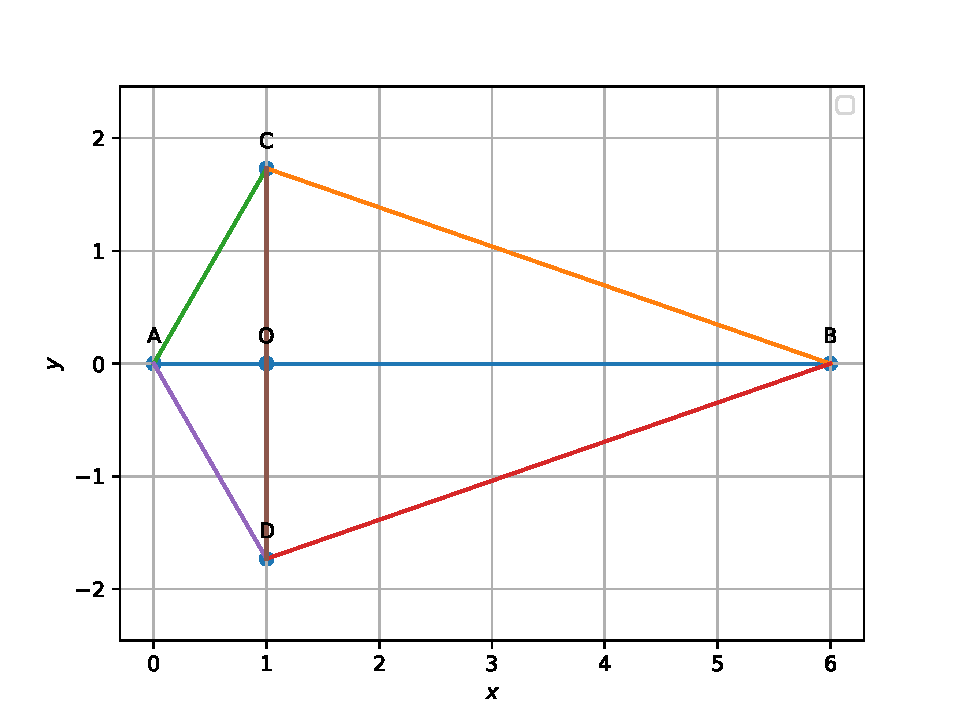
\includegraphics[width=0.75\columnwidth]{chapters/9/9/3/4/figs/figa6.pdf}
		\caption{}
		\label{fig:9/9/3/4}
  	\end{figure}
	\begin{proof}
		See Fig. 
		\ref{fig:9/9/3/4}. $AO$ and $OB$ are medians of triangles $ADC$ and $BDC$. From 
Appendix	  \ref{prop:two-median-area}, 
		\eqref{eq:9/9/3/4} is trivial.
	\end{proof}


\iffalse

	    \includegraphics[width=0.75\columnwidth]{}
   \section{Solution}
   \textbf{Theory:}\\
In 2 triangles with same base and linesegment cd is bisected at o  
\textbf{To Prove:} Ar(ABC)=Ar(ABD) \\
\textbf{Theorem} : Two triangles on the same base (or equal bases) and having the equal heights are equal in area.
\begin{center}
$\therefore$ Ar($\Delta$ ABC)=Ar($\Delta$ ABD)......(1)\\
Hence, Proved    
\end{center}


\
\textbf{termux commands :}
\begin{lstlisting}
python3 matrix.py
\end{lstlisting}


The input parameters for this construction are 
\begin{center}
\begin{tabular}{|c|c|c|}
	\hline
	\textbf{Symbol}&\textbf{Value}&\textbf{Description}\\
	\hline
	k1&4&length of CD\\
	\hline
	k2&6&length of AB\\
	\hline
 
	\hline
	O&$\
	\begin{pmatrix}
		0 \\
		0 \\
	\end{pmatrix}$%
	&Point O\\
	
	\hline
\end{tabular}
\end{center}
\textbf{To Prove:} Ar(ABC)=Ar(ABD)
  %	\begin{align}
	%		\vec{C} &= \myvec{0 \\ 0}, \vec{E}=\myvec{-5 \\ 3}\\
	%			\vec{F} &= \myvec{3 \\ 0}, \vec{D}=\myvec{-3 \\ 0}
	%	\end{align}
		\begin{center}
	a=A-B\\
	b=C-B\\
	c=B-D\\
	Area of the $\Delta$ABC is given by \\
Ar($\Delta$ABC) =$\frac{1}{2}$$\norm{\vec{a}\times\vec{b}}$............(2)\\
    b=C-B\\
	c=B-D\\
		Area of the $\Delta$ABD is given by \\
 Ar($\Delta$ABD) =$\frac{1}{2}$$\norm{\vec{c}\times\vec{d}}$...............(3)
	\end{center}
	
	\begin{center}
$\therefore$ Ar(ABC)=Ar(ABD)........(4)\\
	\end{center}
The below python code realizes the above construction:	
\begin{lstlisting}
https://github.com/anirudhkalyan/fwc
\end{lstlisting}
 \section{Construction}
 	\begin{center}
  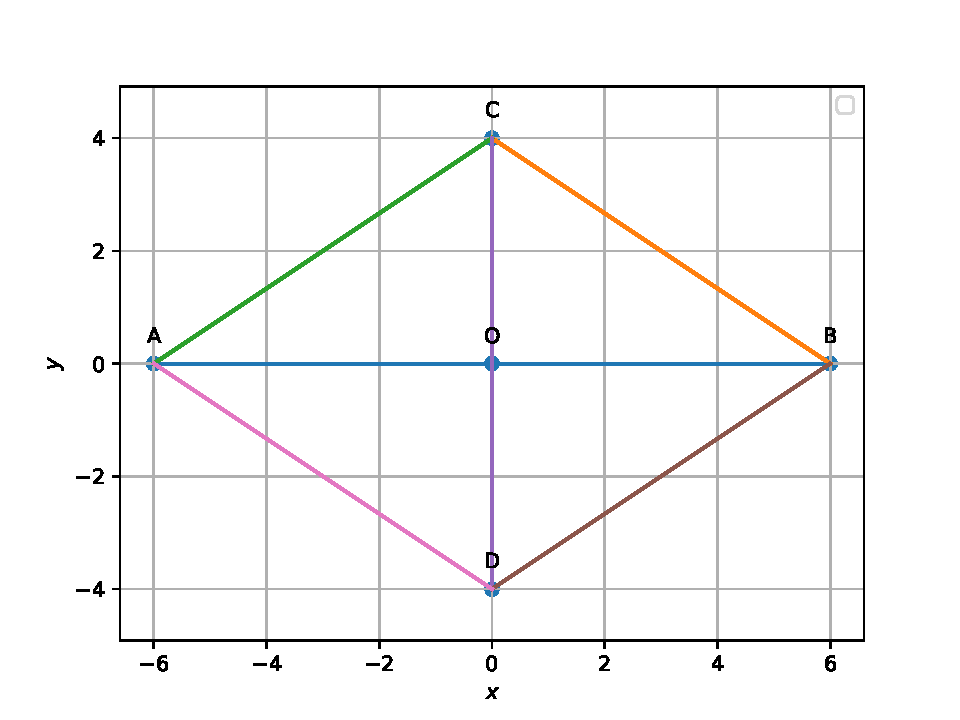
\includegraphics[width=0.75\columnwidth]{figsa1.pdf}
  
  Figure of construction
  	\end{center}
  	  
\bibliographystyle{ieeetr}
\end{document}
\fi

\item 
\label{chapters/9/9/3/4}
\iffalse
\def\mytitle{MATRICES USING PYTHON}
\def\myauthor{P.kalyan}
\def\contact{kalyanpadyalaanirudh@gmail.com}
\def\mymodule{Future Wireless Communication (FWC)}
\documentclass[10pt, a4paper]{article}
\usepackage[a4paper,outer=1.5cm,inner=1.5cm,top=1.75cm,bottom=1.5cm]{geometry}
\twocolumn
\usepackage{graphicx}
\graphicspath{{./images/}}
\usepackage[colorlinks,linkcolor={black},citecolor={blue!80!black},urlcolor={blue!80!black}]{hyperref}
\usepackage[parfill]{parskip}
\usepackage{lmodern}
\usepackage{tikz}
	\usepackage{physics}
%\documentclass[tikz, border=2mm]{standalone}
\usepackage{karnaugh-map}
%\documentclass{article}
\usepackage{tabularx}
\usepackage{circuitikz}
\usetikzlibrary{calc}
\usepackage{amsmath}
\usepackage{amssymb}
\renewcommand*\familydefault{\sfdefault}
\usepackage{watermark}
\usepackage{lipsum}
\usepackage{xcolor}
\usepackage{listings}
\usepackage{float}
\usepackage{titlesec}
\providecommand{\mtx}[1]{\mathbf{#1}}
\titlespacing{\subsection}{1pt}{\parskip}{3pt}
\titlespacing{\subsubsection}{0pt}{\parskip}{-\parskip}
\titlespacing{\paragraph}{0pt}{\parskip}{\parskip}
\newcommand{\figuremacro}[5]{
    \begin{figure}[H]
        \centering
        \includegraphics[width=0.75\columnwidth]{#2}
        \caption[#3]{\textbf{#3}#4}
        \label{fig:#2}
    \end{figure}
}
\newcommand{\myvec}[1]{\ensuremath{\begin{pmatrix}#1\end{pmatrix}}}
\let\vec\mathbf
\lstset{
frame=single, 
breaklines=true,
columns=fullflexible
}

\thiswatermark{\centering \put(0,-90){
\includegraphics[width=0.75\columnwidth]{iith}} }
\title{\mytitle}
\author{\myauthor\hspace{1em}\\\contact\\FWC22031\hspace{6.5em}IITH\hspace{0.5em}\mymodule\hspace{6em}ASSIGN-5}
\date{}
\begin{document}
	\maketitle
	\tableofcontents
   \section{Problem}
   \fi
   $ABC, ABD$ are 2 triangles on same base $AB$, if line segment $CD$ is bisected by $AB$ at $\vec{O}$, show that 
   \begin{align}
		\label{eq:9/9/3/4}
 ar (ABC) = ar (ABD)  
   \end{align}
	\begin{figure}[H]
		\centering
 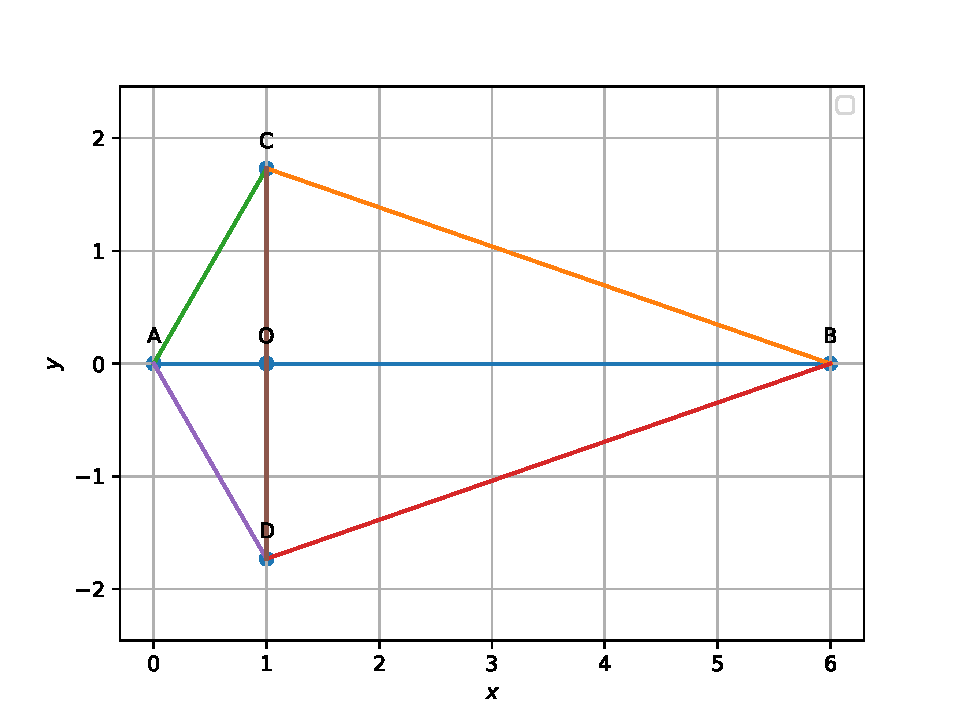
\includegraphics[width=0.75\columnwidth]{chapters/9/9/3/4/figs/figa6.pdf}
		\caption{}
		\label{fig:9/9/3/4}
  	\end{figure}
	\begin{proof}
		See Fig. 
		\ref{fig:9/9/3/4}. $AO$ and $OB$ are medians of triangles $ADC$ and $BDC$. From 
Appendix	  \ref{prop:two-median-area}, 
		\eqref{eq:9/9/3/4} is trivial.
	\end{proof}


\iffalse

	    \includegraphics[width=0.75\columnwidth]{}
   \section{Solution}
   \textbf{Theory:}\\
In 2 triangles with same base and linesegment cd is bisected at o  
\textbf{To Prove:} Ar(ABC)=Ar(ABD) \\
\textbf{Theorem} : Two triangles on the same base (or equal bases) and having the equal heights are equal in area.
\begin{center}
$\therefore$ Ar($\Delta$ ABC)=Ar($\Delta$ ABD)......(1)\\
Hence, Proved    
\end{center}


\
\textbf{termux commands :}
\begin{lstlisting}
python3 matrix.py
\end{lstlisting}


The input parameters for this construction are 
\begin{center}
\begin{tabular}{|c|c|c|}
	\hline
	\textbf{Symbol}&\textbf{Value}&\textbf{Description}\\
	\hline
	k1&4&length of CD\\
	\hline
	k2&6&length of AB\\
	\hline
 
	\hline
	O&$\
	\begin{pmatrix}
		0 \\
		0 \\
	\end{pmatrix}$%
	&Point O\\
	
	\hline
\end{tabular}
\end{center}
\textbf{To Prove:} Ar(ABC)=Ar(ABD)
  %	\begin{align}
	%		\vec{C} &= \myvec{0 \\ 0}, \vec{E}=\myvec{-5 \\ 3}\\
	%			\vec{F} &= \myvec{3 \\ 0}, \vec{D}=\myvec{-3 \\ 0}
	%	\end{align}
		\begin{center}
	a=A-B\\
	b=C-B\\
	c=B-D\\
	Area of the $\Delta$ABC is given by \\
Ar($\Delta$ABC) =$\frac{1}{2}$$\norm{\vec{a}\times\vec{b}}$............(2)\\
    b=C-B\\
	c=B-D\\
		Area of the $\Delta$ABD is given by \\
 Ar($\Delta$ABD) =$\frac{1}{2}$$\norm{\vec{c}\times\vec{d}}$...............(3)
	\end{center}
	
	\begin{center}
$\therefore$ Ar(ABC)=Ar(ABD)........(4)\\
	\end{center}
The below python code realizes the above construction:	
\begin{lstlisting}
https://github.com/anirudhkalyan/fwc
\end{lstlisting}
 \section{Construction}
 	\begin{center}
  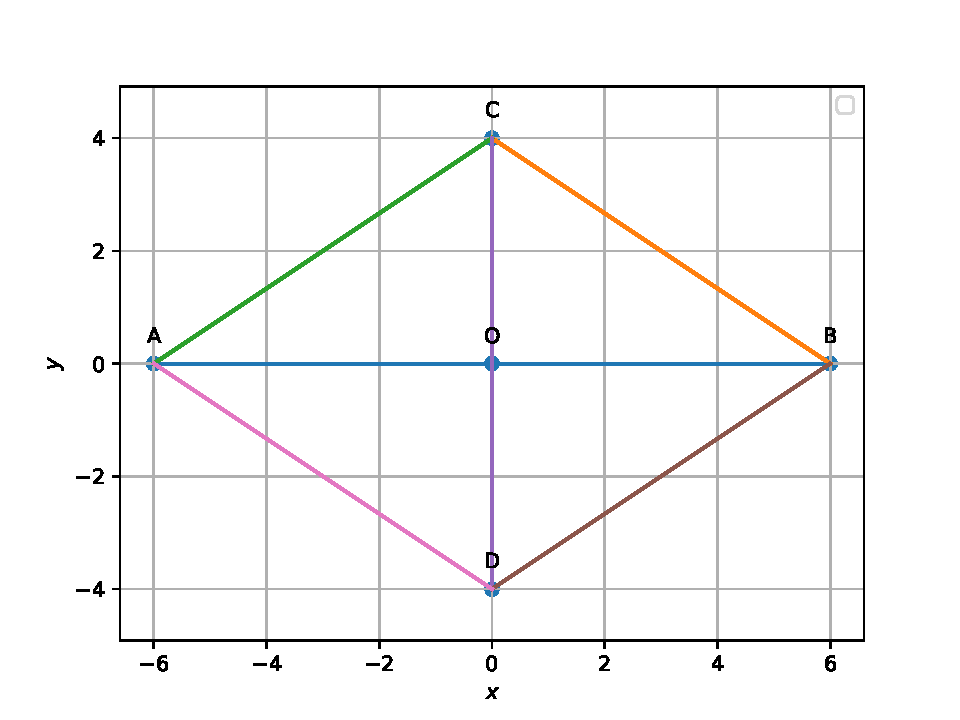
\includegraphics[width=0.75\columnwidth]{figsa1.pdf}
  
  Figure of construction
  	\end{center}
  	  
\bibliographystyle{ieeetr}
\end{document}
\fi

\item 
\label{chapters/9/9/3/4}
\iffalse
\def\mytitle{MATRICES USING PYTHON}
\def\myauthor{P.kalyan}
\def\contact{kalyanpadyalaanirudh@gmail.com}
\def\mymodule{Future Wireless Communication (FWC)}
\documentclass[10pt, a4paper]{article}
\usepackage[a4paper,outer=1.5cm,inner=1.5cm,top=1.75cm,bottom=1.5cm]{geometry}
\twocolumn
\usepackage{graphicx}
\graphicspath{{./images/}}
\usepackage[colorlinks,linkcolor={black},citecolor={blue!80!black},urlcolor={blue!80!black}]{hyperref}
\usepackage[parfill]{parskip}
\usepackage{lmodern}
\usepackage{tikz}
	\usepackage{physics}
%\documentclass[tikz, border=2mm]{standalone}
\usepackage{karnaugh-map}
%\documentclass{article}
\usepackage{tabularx}
\usepackage{circuitikz}
\usetikzlibrary{calc}
\usepackage{amsmath}
\usepackage{amssymb}
\renewcommand*\familydefault{\sfdefault}
\usepackage{watermark}
\usepackage{lipsum}
\usepackage{xcolor}
\usepackage{listings}
\usepackage{float}
\usepackage{titlesec}
\providecommand{\mtx}[1]{\mathbf{#1}}
\titlespacing{\subsection}{1pt}{\parskip}{3pt}
\titlespacing{\subsubsection}{0pt}{\parskip}{-\parskip}
\titlespacing{\paragraph}{0pt}{\parskip}{\parskip}
\newcommand{\figuremacro}[5]{
    \begin{figure}[H]
        \centering
        \includegraphics[width=0.75\columnwidth]{#2}
        \caption[#3]{\textbf{#3}#4}
        \label{fig:#2}
    \end{figure}
}
\newcommand{\myvec}[1]{\ensuremath{\begin{pmatrix}#1\end{pmatrix}}}
\let\vec\mathbf
\lstset{
frame=single, 
breaklines=true,
columns=fullflexible
}

\thiswatermark{\centering \put(0,-90){
\includegraphics[width=0.75\columnwidth]{iith}} }
\title{\mytitle}
\author{\myauthor\hspace{1em}\\\contact\\FWC22031\hspace{6.5em}IITH\hspace{0.5em}\mymodule\hspace{6em}ASSIGN-5}
\date{}
\begin{document}
	\maketitle
	\tableofcontents
   \section{Problem}
   \fi
   $ABC, ABD$ are 2 triangles on same base $AB$, if line segment $CD$ is bisected by $AB$ at $\vec{O}$, show that 
   \begin{align}
		\label{eq:9/9/3/4}
 ar (ABC) = ar (ABD)  
   \end{align}
	\begin{figure}[H]
		\centering
 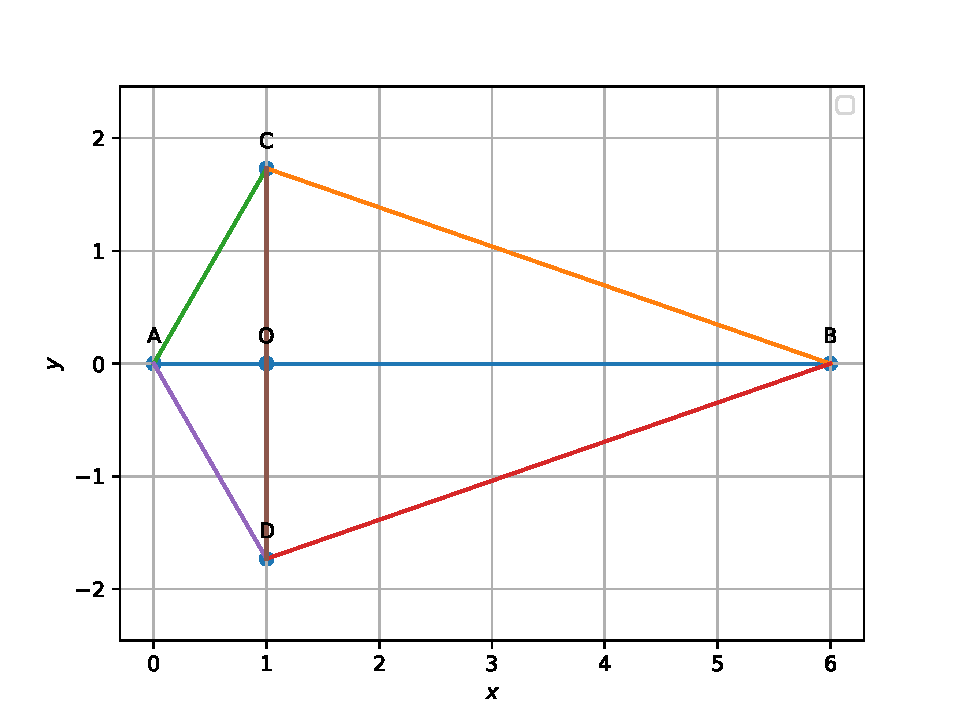
\includegraphics[width=0.75\columnwidth]{chapters/9/9/3/4/figs/figa6.pdf}
		\caption{}
		\label{fig:9/9/3/4}
  	\end{figure}
	\begin{proof}
		See Fig. 
		\ref{fig:9/9/3/4}. $AO$ and $OB$ are medians of triangles $ADC$ and $BDC$. From 
Appendix	  \ref{prop:two-median-area}, 
		\eqref{eq:9/9/3/4} is trivial.
	\end{proof}


\iffalse

	    \includegraphics[width=0.75\columnwidth]{}
   \section{Solution}
   \textbf{Theory:}\\
In 2 triangles with same base and linesegment cd is bisected at o  
\textbf{To Prove:} Ar(ABC)=Ar(ABD) \\
\textbf{Theorem} : Two triangles on the same base (or equal bases) and having the equal heights are equal in area.
\begin{center}
$\therefore$ Ar($\Delta$ ABC)=Ar($\Delta$ ABD)......(1)\\
Hence, Proved    
\end{center}


\
\textbf{termux commands :}
\begin{lstlisting}
python3 matrix.py
\end{lstlisting}


The input parameters for this construction are 
\begin{center}
\begin{tabular}{|c|c|c|}
	\hline
	\textbf{Symbol}&\textbf{Value}&\textbf{Description}\\
	\hline
	k1&4&length of CD\\
	\hline
	k2&6&length of AB\\
	\hline
 
	\hline
	O&$\
	\begin{pmatrix}
		0 \\
		0 \\
	\end{pmatrix}$%
	&Point O\\
	
	\hline
\end{tabular}
\end{center}
\textbf{To Prove:} Ar(ABC)=Ar(ABD)
  %	\begin{align}
	%		\vec{C} &= \myvec{0 \\ 0}, \vec{E}=\myvec{-5 \\ 3}\\
	%			\vec{F} &= \myvec{3 \\ 0}, \vec{D}=\myvec{-3 \\ 0}
	%	\end{align}
		\begin{center}
	a=A-B\\
	b=C-B\\
	c=B-D\\
	Area of the $\Delta$ABC is given by \\
Ar($\Delta$ABC) =$\frac{1}{2}$$\norm{\vec{a}\times\vec{b}}$............(2)\\
    b=C-B\\
	c=B-D\\
		Area of the $\Delta$ABD is given by \\
 Ar($\Delta$ABD) =$\frac{1}{2}$$\norm{\vec{c}\times\vec{d}}$...............(3)
	\end{center}
	
	\begin{center}
$\therefore$ Ar(ABC)=Ar(ABD)........(4)\\
	\end{center}
The below python code realizes the above construction:	
\begin{lstlisting}
https://github.com/anirudhkalyan/fwc
\end{lstlisting}
 \section{Construction}
 	\begin{center}
  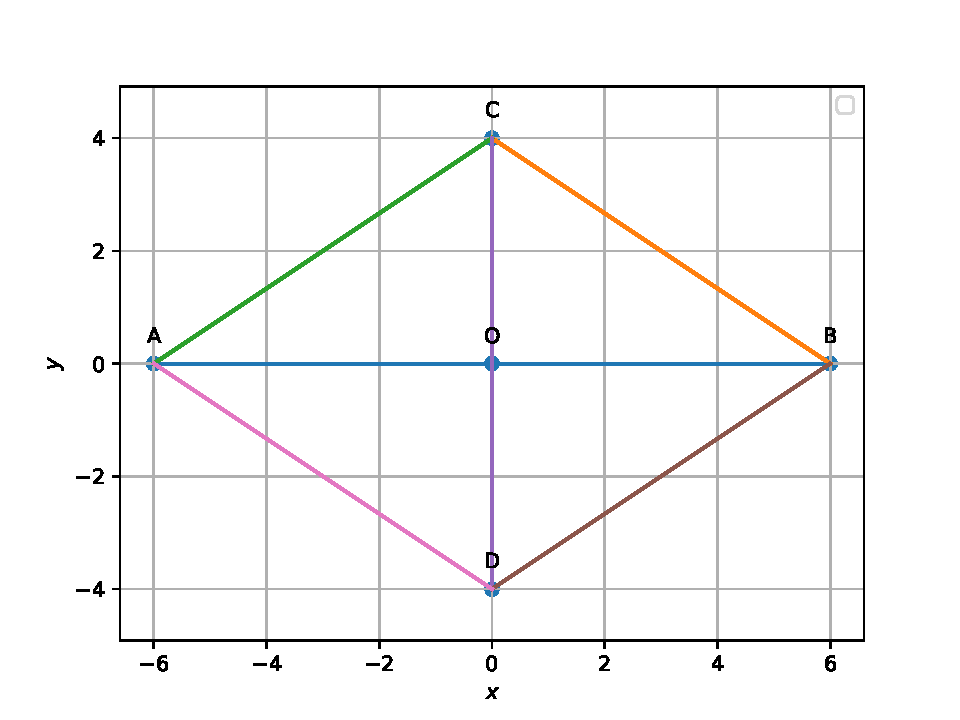
\includegraphics[width=0.75\columnwidth]{figsa1.pdf}
  
  Figure of construction
  	\end{center}
  	  
\bibliographystyle{ieeetr}
\end{document}
\fi

\fi

\end{enumerate}

\item Balance the following chemical equation.
%
\begin{align}
\label{eq:chem_balance}
Fe+H_2O &\rightarrow Fe_3O_4 + H_2
\end{align}
%\solution 
%\begin{enumerate}[label=\thesection.\arabic*,ref=\thesection.\theenumi]
\numberwithin{equation}{enumi}
\numberwithin{figure}{enumi}
\numberwithin{table}{enumi}
\item 
\item 
\item 
\label{chapters/9/9/4/3}
\iffalse
\documentclass[10pt,a4paper]{report}
\usepackage[utf8]{inputenc}
\usepackage{amsmath}
\usepackage{amsfonts}
\usepackage{amssymb}
\usepackage{graphicx}
\usepackage{multicol}
\usepackage{tabularx}
\usepackage{tikz}
\newcommand{\myvec}[1]{\ensuremath{\begin{pmatrix}#1\end{pmatrix}}}
\let\vec\mathbf
\let\myvec\bf
\providecommand{\mtx}[1]{\mathbf{#1}}
\newcommand{\mydet}[1]{\ensuremath{\begin{vmatrix}#1\end{vmatrix}}}
\usetikzlibrary{arrows,shapes,automata,petri,positioning,calc}
\usepackage{hyperref}
\usepackage{tikz}
\usetikzlibrary{matrix,calc}
\usepackage[margin=0.5in]{geometry}
\providecommand{\norm}[1]{\left\lVert#1\right\rVert}
\let\vec\mathbf
\newenvironment{Figure}
  {\par\medskip\noindent\minipage{\linewidth}}
  {\endminipage\par\medskip}
    
 
 
\begin{document}
%--------------------logo figure-------------------------%
\begin{figure*}[!tbp]
  \centering
  \begin{minipage}[b]{0.4\textwidth}
    \end{minipage}
  \hfill
  \vspace{5mm}\begin{minipage}[b]{0.4\textwidth}

  \end{minipage}\vspace{0.2cm}
\end{figure*}
%--------------------name & rollno-----------------------
\raggedright \textbf{Name}:\hspace{1mm} Varsha Reddy\hspace{3cm} \Large \textbf{Assignment-4}\hspace{2.5cm} % 
\normalsize \textbf{Roll No.} :\hspace{1mm} FWC22038\vspace{1cm}
\begin{multicols}{2}

\raggedright \textbf{PROBLEM:}\vspace{2mm}\\
\fi
In Fig.
		\ref{fig:9/9/4/3}
	\begin{figure}[H]
		\centering
 \includegraphics[width=0.75\columnwidth]{chapters/9/9/4/3/figs/ABC.pdf}
		\caption{}
		\label{fig:9/9/4/3}
  	\end{figure}
	$ABCD, DCFE$ and $ABFE$ are parallelograms. Show that   
	\begin{align}
	ar(ADE) = ar(BCF)
		\label{eq:9/9/4/3}
	\end{align}
	\begin{proof}
		From the given information and Appendix
	  \ref{eq:two-pgm},
  \begin{align}
		\label{eq:9/9/4/3/1}
	  \vec{B}-\vec{A} &= \vec{C} -\vec{D}
	  \\
		\label{eq:9/9/4/3/2}
	  \vec{C}-\vec{D} &= \vec{F} -\vec{E}
	  \\
		\label{eq:9/9/4/3/3}
	  \vec{B}-\vec{A} &= \vec{F} -\vec{E}
  \end{align}
  Thus, from  Appendix
  \ref{prop:pgm2d},
\begin{align}
	ar(ADE)  &= 
	\norm{\brak{\vec{D}-\vec{E}} \times \brak{\vec{D}-\vec{A}}}
	\\
	& = 
	\norm{\brak{\vec{C}-\vec{F}} \times \brak{\vec{C}-\vec{B}}}
	\\
	&=	ar(ADE) 
  \end{align}
  upon substituting from 
		\eqref{eq:9/9/4/3/1}
		and 
		\eqref{eq:9/9/4/3/2}.
	\end{proof}
	\iffalse
\vspace{0.5cm}\raggedright \\
Theory:
Parallelograms on the same base and in between the same parallels are equal in area.\\
Given: ABCD,DCFE and ABFE are parallelograms.
\vspace{2mm} \\ 
%----------------Solution  statement--------------%
\raggedright \textbf{Solution Statement:}\vspace{2mm}
\raggedright \\We can see that the sides of a triangle ADE and BCF are also the opposite sides of a given parallelogram. Now we can show both the triangles are congruent using congruency property. We know that congruent triangles are equal areas.  \\
\vspace{5mm}
\section{Construction}
  \begin{center}
   %\includegraphics[width=0.75\columnwidth]{assignment4/ABC.pdf}
     \includegraphics[width=0.75\columnwidth]{ABC.pdf} 
     Figure of Construction
   \end{center}
   \vspace{5mm}

\section{Table :}

The input parameters for this construction are 
\begin{center}
\begin{tabular}{|c|c|c|}
	\hline
	\textbf{Symbol}&\textbf{Value}&\textbf{Description}\\
	\hline
	a&3&EA\\
	\hline
	b&4.5&EF\\
	\hline
	c&2&ED\\
	\hline
	${\theta}_1$& 1$\pi/3$&$ \angle $AEF\\ 
	\hline
	${\theta}_2$& 2$\pi/3$&$ \angle $DEF\\ 
	    \hline
	E&$\
	\begin{pmatrix}
		0 \\
		0 \\
	\end{pmatrix}$%
	&Point E\\
	\hline
\end{tabular}
\end{center}

1. Considering point 'E' as origin.\\
2. From E,with some angle of 60 degrees,mark the point 'A'.\\
3. From E,with some angle of 120 degrees,mark the point 'D'.\\
4. With the distance of 'b' locate the point 'F'.\\
5. To locate a point 'B'\\
\begin{center}
    \myvec{ B = A+F-E }
\end{center}
6. To locate a point 'C'\\
\begin{center}
    \myvec{ C = D+F-E }
\end{center}
7. Joining all the lines from the figure.
\vspace{0.5cm}\\
%-----------------------------solution---------------------------
 \section{Solution}
% \vspace{2mm}\\
n ABCD,
\begin{equation}
\vec{A-B}=\vec{D-C}
\end{equation}
\begin{equation}
\vec{A-D}=\vec{B-C}
\end{equation}
\\
In DEFC,
\begin{equation}
\vec{D-C}=\vec{E-F}
\end{equation}
\begin{equation}
\vec{D-E}=\vec{C-F}
\end{equation}
\\
In ABEF,
\begin{equation}
\vec{A-B}=\vec{E-F}
\end{equation}
\begin{equation}
\vec{A-E}=\vec{B-F}
\end{equation}

\vspace{1mm}

\textbf{To Prove:} 
  \begin{center}
  \begin{equation}
      \vec{Ar(ADE)=Ar(BCF)}
  \end{equation}
 \vspace{3mm}
 Area of the triangle $\Delta$ADE is given by \\
 Ar($\Delta$ADE) 
\begin{equation} 
 = \frac{1}{2}\norm{\vec{A-D}\times\vec{D-E}}
\end{equation}
  %\vspace{3mm}
 \vspace{3mm}
  Area of the triangle $\Delta$BCF is given by \\
  Ar($\Delta$BCF)
   \begin{equation}
   =\frac{1}{2}\norm{\vec{B-C}\times\vec{C-F}}
   \end{equation}
 \end{center}
 substituiting (2) and (4) in (9),
 \begin{equation}
   =\frac{1}{2}\norm{\vec{A-D}\times\vec{D-E}}
   \end{equation}
   from (8) and (10),
 \begin{center}
\begin{equation}
    \vec{Ar(ADE)=Ar(BCF)}
\end{equation}
\end{center}
The below python code realizes the above construction: \\
\url{https://github.com/9705701645/FWC/blob/main/lines4.py}
\bibliographystyle{ieeetr}
\end{multicols}
\end{document}
\fi


\item 
\label{chapters/9/9/4/4}
\iffalse
%\documentclass{article}
\documentclass[journal,12pt,twocolumn]{IEEEtran}

% Language setting
% Replace `english' with e.g. `spanish' to change the document language
\usepackage[english]{babel}

% Set page size and margins
% Replace `letterpaper' with `a4paper' for UK/EU standard size
%%\usepackage[letterpaper,top=2cm,bottom=2cm,left=3cm,right=3cm,marginparwidth=1.75cm]{geometry}

% Useful packages
\usepackage[utf8]{inputenc}
\usepackage{enumitem}
\usepackage{multicol}
\usepackage{ragged2e}
\usepackage{amsmath}
\usepackage{amssymb}
\usepackage{graphicx}
\let\vec\mathbf
\let\myvec\bf
\usepackage{array}
\usepackage{blindtext}
%\usepackage[paperwidth=10cm]{geometry}
\usepackage{tkz-euclide}
%\usepackage{tikz}
\usetikzlibrary{
  circuits.logic,
  circuits.logic.US,
  positioning
}
\usepackage[colorlinks=true, allcolors=blue]{hyperref}

\title{Line Assignment}
\author{Navya Valmeekam}
\let\vec\mathbf
\begin{document}
\providecommand{\norm}[1]{\left\lVert#1\right\rVert}
\maketitle
\begin{tableofcontents}
\section{Problem}
\fi
In figure below, $ABCD$ is a parallelogram and $BC$ is produced to a point $\vec{Q}$ such that $AD = CQ$. If $AQ$ intersect $DC$ at $\vec{P}$, show that 
	\begin{align}
	ar (BPC) = ar (DPQ).
		\label{eq:9/9/4/4}
	\end{align}
	\begin{figure}[!h]
		\centering
 \includegraphics[width=\columnwidth]{chapters/9/9/4/4/figs/construction.png}
		\caption{}
		\label{fig:9/9/4/4}
  	\end{figure}
	\iffalse
[Hint : Join AC.]\\
\includegraphics[scale=0.4]
\begin{center}
Figure of Construction
\end{center}
\section{Construction}
\begin{center}
\begin{tabular}{|c|c|c|}
\hline
\textbf{Symbol}&{Value}&{Description}\\
\hline
r1&5&DA\\
\hline
r2&8&DC\\
\hline
${\theta}_1$& 2$\pi/5$&$ \angle $ADC\\ 
\hline
\end{tabular}
\end{center}
\begin{center}
\begin{equation}
\vec{B}= \vec{A}+\vec{C}-\vec{D}
\end{equation}
\begin{equation}
\vec{Q}= \vec{D}+\vec{C}-\vec{A}
\end{equation}
\begin{equation}
\vec{P}= \vec{(D+C)/2}
\end{equation}
\end{center}
%\end{abstract}
\section{Solution}
\justify
\textbf{Construction: Join AC}\\
\justify
\textbf{To Prove:}
ar($\Delta$ BPC) = ar($\Delta$ DPQ)\\
\\
We need to prove that ar(BPC)=ar(DPQ)\\
\\
Given BC is extended to Q, so \begin{equation}
\vec{AD} \: || \: \vec{CQ} 
\end{equation}
and given \begin{equation}
\vec{AD}=\vec{CQ}
\end{equation}
from (4) and (5), ACQD is a parallelogram\\
\\
In ABCD,
\begin{equation}
\vec{A-B}=\vec{D-C}
\end{equation}
\begin{equation}
\vec{A-D}=\vec{B-C}
\end{equation}
\\
In ACQD,
\begin{equation}
\vec{A-C}=\vec{D-Q}
\end{equation}
\begin{equation}
\vec{A-D}=\vec{C-Q}
\end{equation}
Area of triangle BPC \\
\begin{equation}
=\vec{1/2} \vec{x} \norm{(\vec{P} - \vec{C}) \times (\vec{B} - \vec{C})}
\end{equation}
Substituiting (3) in (10),\\
\begin{equation}
=\vec{1/2} \vec{x} \norm{(\frac{\vec{D}-\vec{C}}{2}) \times (\vec{B} - \vec{C})}
\end{equation}
\begin{equation}
=\vec{1/4} \vec{x} \norm{(\vec{D-C}) \times (\vec{B-C})}
\end{equation}\\
\\
Area of triangle DPQ\\
\begin{equation}
=\vec{1/2} \vec{x} \norm{(\vec{D} - \vec{P}) \times (\vec{Q} - \vec{D})}
\end{equation}
Substituiting (3) in (13),\\
\begin{equation}
=\vec{1/2} \vec{x} \norm{(\frac{\vec{D}-\vec{C}}{2}) \times (\vec{Q} - \vec{D})}
\end{equation}
from (6),
\begin{equation}
\vec{C-A}=\vec{Q-D}
\end{equation}
And from $\Delta$ ABC,
\begin{equation}
\vec{C-A}=\vec{A-B}+\vec{B-C}
\end{equation}
Substituiting (15) and (16) in (14),\\
\begin{equation}
=\vec{1/4} \vec{x} \norm{(\vec{D}-\vec{C}) \times ((\vec{A} - \vec{B})+(\vec{B}-\vec{C}))}
\end{equation}
\begin{equation}
=\vec{1/4} \vec{x} \norm{((\vec{D}-\vec{C}) \times (\vec{A} - \vec{B}))+((\vec{D}-\vec{C}) X (\vec{B}-\vec{C}))}
\end{equation}
Substituiting (6) in (18),\\
\begin{equation}
=\vec{1/4} \vec{x} \norm{((\vec{A}-\vec{B}) \times (\vec{A} - \vec{B}))+((\vec{D}-\vec{C}) X (\vec{B}-\vec{C}))}
\end{equation}
\begin{equation}
=\vec{1/4} \vec{x} \norm{(\vec{D-C}) \times (\vec{B-C})}
\end{equation}\\
from (12) and (20),\\
\begin{align*}
\vec{ar(\Delta BPC) = ar(\Delta DPQ)}
\end{align*}
\\
hence proved
%\end{flushleft}
\end{tableofcontents}
\end{document}
\fi

\item 
\label{chapters/9/9/4/5}
\iffalse
\def\mytitle{MATRICES USING PYTHON}
\def\myauthor{VAMSI SUNKARI}
\def\contact{vamsisunkari9849@gmail.com}
\def\mymodule{Future Wireless Communication (FWC)}
\documentclass[10pt, a4paper]{article}
\usepackage[a4paper,outer=1.5cm,inner=1.5cm,top=1.75cm,bottom=1.5cm]{geometry}
\twocolumn
\usepackage{graphicx}
\graphicspath{{./images/}}
\usepackage[colorlinks,linkcolor={black},citecolor={blue!80!black},urlcolor={blue!80!black}]{hyperref}
\usepackage[parfill]{parskip}
\usepackage{lmodern}
\usepackage{tikz}
 \usepackage{physics}
\usepackage{karnaugh-map}
\usepackage{setspace}
\doublespacing
%\documentclass{article}
\usepackage{tabularx}
%\usepackage{circuitikz}
\usetikzlibrary{calc}
\usepackage{amsmath}
\usepackage{amssymb}
\renewcommand*\familydefault{\sfdefault}
%\usepackage{watermark}
\usepackage{lipsum}
\usepackage{xcolor}
\usepackage{listings}
\usepackage{float}
\usepackage{titlesec}
\providecommand{\mtx}[1]{\mathbf{#1}}
\titlespacing{\subsection}{1pt}{\parskip}{3pt}
\titlespacing{\subsubsection}{0pt}{\parskip}{-\parskip}
\titlespacing{\paragraph}{0pt}{\parskip}{\parskip}
\newcommand{\figuremacro}[5]{
    \begin{figure}[#1]
        \centering
        \includegraphics[width=#5\columnwidth]{#2}
        \caption[#3]{\textbf{#3}#4}
        \label{fig:#2}
    \end{figure}
}
\newcommand{\myvec}[1]{\ensuremath{\begin{pmatrix}#1\end{pmatrix}}}
\let\vec\mathbf
\lstset{
frame=single, 
breaklines=true,
columns=fullflexible
}
\title{\mytitle}
\author{\myauthor\hspace{1em}\\\contact\\FWC22040\hspace{6.5em}IITH\hspace{0.5em}\mymodule\hspace{6em}ASSIGN-5}
\date{}
\begin{document}
 \maketitle
 \tableofcontents
   \section{Problem}
   \fi
   In Fig. 
		\ref{fig:9/9/4/5},
	\begin{figure}[!h]
		\centering
 \includegraphics[width=\columnwidth]{chapters/9/9/4/5/figs/matrix.png}
		\caption{}
		\label{fig:9/9/4/5}
  	\end{figure}
$  ABC$ and $BDE$ are two equilateral
triangles such that $\vec{D}$ is the mid-point of $BC$. If $AE$
intersects $BC$ at $\vec{F}$, show that
\begin{align}
	ar(BDE) &=\frac{1}{4} ar(ABC)\\
	ar(BDE) &=\frac{1}{2} ar(BAE)\\
ar(ABC) &=2 ar(BEC)\\
ar(BFE) &= ar(AFD)\\
ar(BFE) &=2ar(FED)\\
	ar(FED) &=\frac{1}{8} ar(AFC)
\end{align}
\iffalse


\begin{proof}
From Appendix
    \ref{prop:two-isosc}, considering $\triangle$s $ABC$ and $EBD$,
\begin{align}
		\label{fig:9/9/4/5/b}
	\brak{\vec{B}-\vec{C}}^{\top}
	\brak{\vec{A}-\vec{D}} &=\vec{0}
	%\brak{\vec{A}-\frac{\vec{B}+\vec{C}}{2}}&=\vec{0}
	\\
	\brak{\vec{B}-\vec{D}}^{\top}
	\brak{\vec{E}-\frac{\vec{B}+\vec{D}}{2}}&=\vec{0}
		\label{fig:9/9/4/5/e}
\end{align}
		\eqref{fig:9/9/4/5/e}
		can be expressed as
\begin{align}
	\brak{\vec{B}-\vec{D}}^{\top}
	%\brak{\vec{B}-\brak{\frac{\vec{B}+\vec{C}}{2}}}^{\top}
	\brak{\vec{E}-\frac{\vec{B}+\vec{D}}{2}}&=\vec{0}
	%\brak{\vec{E}-\frac{\vec{B}+\brak{\frac{\vec{B}+\vec{C}}{2}}}{2}}&=\vec{0}
	\\
	\implies \brak{\vec{B}-\vec{C}}^{\top}
	\brak{\vec{E}-\frac{\vec{B}+\vec{D}}{2}}&=\vec{0}
%	\brak{\vec{E}-\frac{3\vec{B}+2\vec{C}}{2}}&=\vec{0}
		\label{fig:9/9/4/5/e/2}
\end{align}
upon substituting
\begin{align}
	\vec{D}=\frac{\vec{B}+\vec{C}}{2}
\end{align}
From 
		\eqref{fig:9/9/4/5/b},
		\eqref{fig:9/9/4/5/e/2}
		and 
	  Appendix \ref{prop:two-orth-para},
\begin{align}
	\vec{E}-\frac{\vec{B}+\vec{D}}{2}&=
	k\brak{\vec{A}-\vec{D}}
	%\vec{E}-\frac{3\vec{B}+2\vec{C}}{2}&=
	%k\brak{\vec{A}-\brak{\frac{\vec{B}+\vec{C}}{2}}}
	\\
\implies
	\vec{E} &= \frac{\vec{B}+\vec{D}}{2}+k\brak{\vec{A}-\vec{D}}
	%\frac{3\vec{B}+2\vec{C}}{2}+	k\brak{\vec{A}-\brak{\frac{\vec{B}+\vec{C}}{2}}}
	%\vec{E} &= \frac{3\vec{B}+2\vec{C}}{2}+	k\brak{\vec{A}-\brak{\frac{\vec{B}+\vec{C}}{2}}}
		\label{fig:9/9/4/5/ef}
\end{align}
Since
\begin{align}
	\vec{E} \times \vec{B} &=\frac{\vec{D}\times \vec{B}}{2}+k\brak{\vec{A}-\vec{D}} \times \vec{B}
	\\
	&=\brak{\frac{1}{2}-k}\vec{D}\times \vec{B}+k\vec{A} \times \vec{B}
	%\vec{E} \times \vec{B} &=\brak{\frac{3\vec{B}+2\vec{C}}{2}+k\brak{\vec{A}-\brak{\frac{\vec{B}+\vec{C}}{2}}}} \times \vec{B}
%	\\
%	&=\brak{\vec{C}+k\brak{\vec{A}-\brak{\frac{\vec{C}}{2}}}} \times \vec{B}
%	\\
%	\vec{B} \times \vec{D} &=\vec{B} \times \frac{\vec{B}+\vec{C}}{2}
%	\\
%	&=\vec{B} \times \frac{\vec{C}}{2}
	\\
	\vec{D} \times \vec{E}&=\frac{\vec{D}\times\vec{B}}{2}+k \vec{D}\times\vec{A}
	%\vec{D} \times \vec{E}&=\brak{\frac{\vec{B}+\vec{C}}{2}}\times\brak{\frac{3\vec{B}+2\vec{C}}{2}+	k\brak{\vec{A}-\brak{\frac{\vec{B}+\vec{C}}{2}}}}
\end{align}
	upon substituting from 
		\eqref{fig:9/9/4/5/ef},
\begin{align}
		\label{fig:9/9/4/5/e/area}
{\vec{E} \times \vec{B}+\vec{B} \times \vec{D}+\vec{D} \times \vec{E}}
 \\
= 
k\brak{\vec{A} \times \vec{B}+\vec{B} \times \vec{D}+\vec{D} \times \vec{A}}
%	\\
%	+\vec{B} \times \vec{D}+\vec{D} \times \brak{\frac{3\vec{B}+2\vec{C}}{2}+k\brak{\vec{A}-\brak{\frac{\vec{B}+\vec{C}}{2}}}}
\end{align}
%upon  substituting from 
%		\eqref{fig:9/9/4/5/ef}
		%in
		%\eqref{fig:9/9/4/5/e/area},
\end{proof}
%\iffalse
From 
	  \eqref{eq:two-tri-indep},
\begin{align}
	  \brak{p+q}\vec{E}- p\vec{B} -q\vec{D} &= 0
	  \\
	  \implies
	  \brak{p+q}\brak{\frac{\vec{B}+\vec{D}}{2}+k\brak{\vec{A}-\vec{D}}}- p\vec{B} -q\vec{D} &= 0
	  \\
	  \text{or, }
	  \brak{\frac{q-p}{2}}\vec{B}+\brak{\frac{p-q}{2}-k\brak{p+q}}\vec{D}+k\vec{A}&= 0
\end{align}
Since $\vec{D}$ is the mid point of $BC$, substituting 
in the above,
\begin{align}
	\brak{\frac{q-p}{2}}\vec{B}+\brak{\frac{p-q}{2}-k\brak{p+q}}\brak{\frac{\vec{B}+\vec{C}}{2}}+k\vec{A}&= 0
%	\brak{\frac{q-p}{2}}\vec{B}-\brak{q+k\brak{{\frac{p+q}{2}}}}\frac{\vec{B}+\vec{C}}{2}+k\brak{p+q}\vec{A}&= 0
%	  \\
%	  \implies
%k\brak{p+q}\vec{A}+
%	\brak{\frac{q-p}{2}-\brak{q+k\brak{{\frac{p+q}{2}}}}}\vec{B}-\brak{q+k\brak{{\frac{p+q}{2}}}}\frac{\vec{B}+\vec{C}}{2}+k\brak{p+q}\vec{A}&= 0
	\\
	\implies 
	k\vec{A}+\brak{\frac{q-p}{2}}\vec{B}+\brak{\frac{p-q}{2}-k\brak{p+q}}\brak{\frac{\vec{B}+\vec{C}}{2}}&= 0
\end{align}
in the above, 

[Hint : Join EC and AD. Show that BE  AC abd DE AB, etc.]

   %  \includegraphics[scale=1.0]{diag_1.png}
   \section{Solution}
   \textbf{Theory:}\\
   \textbf{To Prove:} ar(BDE)=1/4 ar(ABC) \\
   ABC and BDE are two equilateral triangles such that D is the mid-point of BC.If AE intersets BC at F


\textbf{termux commands :}
\begin{lstlisting}
python3 matrix.py
\end{lstlisting}


The input parameters for this construction are 
\begin{center}
\begin{tabular}{|c|c|c|}
 \hline
 \textbf{Symbol}&\textbf{Value}&\textbf{Description}\\
 \hline
 r&5&AB\\
 \hline

 $\vec{A}$&$r\myvec{\cos\theta \\ \sin\theta}$%
 &Point A\\
 \hline
 $\vec{E}$&$\myvec{\frac{r}{2}\cos\theta \\ \frac{r}{2}\sin\theta}$
 &Point E\\
 \hline
 $\vec{B}$&$\myvec{0 \\ 0}$%
 &Point B\\
 \hline
 $\vec{C}$&$\myvec{r \\ 0}$%
 &Point C\\
 \hline
 $\vec{D}$&$\myvec{r/2 \\ 0}$%
 &Point D\\
 \hline
 $\vec{F}$&$\myvec{\frac{2}{3}r\cos\theta \\ 0}$%
 &Point F\\
 \hline
 ${\theta}_1$& $\pi/3$&$ \angle $ABC\\ 
 \hline
\end{tabular}
\end{center}
\textbf{To Prove:} ar(BDE)=1/4 ar(ABC)
  \begin{center}
 
 $\vec{v1}=\vec{A-B}$\\
 $\vec{v2}=\vec{A-C}$\\

$ar(\Delta ABC) =\frac{1}{2}\norm{\vec{v1}\times\vec{v2}}$............(1)\\
$\vec{v3}=\vec{B-D}$\\
 $\vec{v4}=\vec{B-E}$\\
 
 $ar(\Delta BDE) =\frac{1}{2}\norm{\vec{v3}\times\vec{v4}}$...............(2)\\
 $ar(BDE)= \frac{1}{4} ar(ABC)$
 \end{center}
 \textbf{To Prove:}  ar(BDE)=1/2 ar(BAE) 
 \begin{center}
$\vec{v5}=\vec{A-E}$\\
$\vec{v6}=\vec{A-B}$\\

 $ar(\Delta BAE) =\frac{1}{2}\norm{\vec{v5}\times\vec{v6}}$...............(3)\\
 $ar(BDE)=\frac{1}{2} ar(BAE)$
\end{center}
 \textbf{To Prove:}  ar(ABC)=2 ar(BEC) 
 \begin{center}
 $\vec{v7}=\vec{B-C}$\\
$\vec{v8}=\vec{B-E}$\\

 $ar(\Delta BEC) =\frac{1}{2}\norm{\vec{v7}\times\vec{v8}}$...............(4)\\
 $ar(ABC)=2 ar(BEC)$
 \end{center}
 \textbf{To Prove:}  ar(BFE)=ar(AFD) 
 \begin{center}
 $\vec{v9}=\vec{B-F}$\\
$\vec{v10}=\vec{B-E}$\\
$\vec{v11}=\vec{A-D}$\\
$\vec{v12}=\vec{A-F}$\\
 $ar(\Delta BFE) =\frac{1}{2}\norm{\vec{v9}\times\vec{v10}}$...............(4)\\
 $ar(\Delta AFD) =\frac{1}{2}\norm{\vec{v11}\times\vec{v12}}$...............(4)\\
 ar(BFE)=ar(AFD)
 \end{center}
 \textbf{To prove} : ar(BFE) =2ar(FED)
\begin{center}
$\vec{v13}=\vec{F-E}$\\
$\vec{v14}=\vec{F-D}$\\
 $ar(\Delta FED) =\frac{1}{2}\norm{\vec{v13}\times\vec{v14}}$...............(4)\\
 $ar(BFE) =2ar(FED)$   
\end{center}
\textbf{To prove} : $ar(FED) =\frac{1}{8} ar(AFC)$
\begin{center}
$\vec{v15}=\vec{A-F}$\\
$\vec{v16}=\vec{A-C}$\\
$ar(\Delta AFC) =\frac{1}{2}\norm{\vec{v15}\times\vec{v16}}$...............(4)\\ 
 $ar(FED) =\frac{1}{8} ar(AFC)$   
\end{center}
The below python code realizes the above construction: 
\begin{lstlisting}
https://github.com/Vamsi9849/iithfwc/blob/main/Matrix_line/codes/matrix.py
\end{lstlisting}
 \section{Construction}
  \begin{center}
  \includegraphics[scale=0.39]{par.pdf}  
  Figure of construction
   \end{center}   
\bibliographystyle{ieeetr}
\end{document}
\fi

\item 
\item 
\item 
\end{enumerate}

\item Balance the following chemical equation.
\begin{align}
  \label{matrix/50/eq1}
NaOH + H_2SO_4 \xrightarrow{} Na_2SO_4  +  H_2O
\end{align}
%\\
%\solution
%\input{chapters/chemistry/solutions/5.tex}
%\item Balance the following chemical equation
%\begin{align}\label{1}
%    BaCl_2 + H_2SO_4 \xrightarrow{} BaSO_4 + HCl
%\end{align}
\end{enumerate}
 

